\chapter{Event selection in ND-GAr}
\label{chapter:gar_selection}

\section{Data sample}

{\color{red}
In this section I need to make sure to mention:
\begin{itemize}
    \item I need to comment on the versions of the software that were used for the production of the different samples (if we end up having more than one). The version of \texttt{GENIE} used was 
    \item We use GArG4 instead of \texttt{edep-sim} for the particle propagation. Because both \texttt{Geant4} wrappers use different configurations for the simulation, the results obtained are different. The default \texttt{edep-sim} configuration used by the DUNE ND is appropriate for ND-LAr, where thresholds for particle production are higher. In the case of ND-GAr, these parameters need to be adjusted accordingly. For the time being, in these first productions of analysis files, we will use our standalone \texttt{Geant4} implementation. For future iterations these differences will need to be revisited and understood, so we can use the same simulation workflow as the rest of the ND.
    \item I need to comment on the sample size. The first sample produced was simply $10^{5}$ events inside the HPgTPC volume. There is also the question of the other sample we may want to produce for the $\geq 3\pi^{\pm}$ selection (ask Naseem).
    \item So far we have only simulated single interaction events. Ideally, we should move to simulate full spills. Of course, we need to understand how many interactions we expect in ND-GAr per spill. Also, there is the question of having neutrino interactions happening in the other detector volumes (ECal, magnet, \dots).
    \item At some point, we should generate a sample of rock muons making it to ND-GAr.
    \item I think I should comment on the run plan (at least the part that concerns ND-GAr), and what it means in terms of generating a full production sample. It will be good to have an understanding of the POT we need on-axis and at each off-axis positions (for both FHR and RHC).
\end{itemize}
}

\begin{table}[t]
	\caption{Event rates in ND-GAr.}
	\begin{center}
		\begin{small}
			\begin{tabular}{lcc}
                & \multicolumn{2}{c}{Events/ton/year}                                                                   \\[2mm] \cline{2-3} 
            \multicolumn{1}{c}{\rule{0pt}{1.1\normalbaselineskip}Process}       & $1.1 \times 10^{21} ~ \mathrm{POT}/\mathrm{year}$ & $1.9 \times 10^{21} ~ \mathrm{POT}/\mathrm{year}$ \\[2mm] \hline
            \rule{0pt}{1.1\normalbaselineskip}All $\nu_{\mu}$-CC                & $1.60 \times 10^{6}$                              & $2.83 \times 10^{6}$                              \\[2mm]
            $\hspace{0.5 cm}$ CC $0\pi$       & $5.28 \times 10^{5}$                              & $9.35 \times 10^{5}$                              \\[2mm]
            $\hspace{0.5 cm}$ CC $1\pi^{\pm}$ & $3.02 \times 10^{5}$                              & $5.34 \times 10^{5}$                              \\[2mm]
            $\hspace{0.5 cm}$ CC $1\pi^{0}$   & $1.65 \times 10^{5}$                              & $2.92 \times 10^{5}$                              \\[2mm]
            $\hspace{0.5 cm}$ CC $2\pi$       & $3.18 \times 10^{5}$                              & $5.63 \times 10^{5}$                              \\[2mm]
            $\hspace{0.5 cm}$ CC $3\pi$       & $1.36 \times 10^{5}$                              & $2.41 \times 10^{5}$                              \\[2mm]
            $\hspace{0.5 cm}$ CC other        & $1.52 \times 10^{5}$                              & $2.69 \times 10^{5}$                              \\[2mm] \hline
            \rule{0pt}{1.1\normalbaselineskip}All $\bar{\nu}_{\mu}$-CC          & $7.54 \times 10^{4}$                              & $1.33 \times 10^{5}$                              \\[2mm]
            All NC                            & $5.50 \times 10^{5}$                              & $9.73 \times 10^{5}$                              \\[2mm]
            All $\nu_{e}$-CC                  & $2.70 \times 10^{4}$                              & $4.78 \times 10^{4}$                             
            \end{tabular}
		\end{small}
	\end{center}
	\label{tab:ndgar_event_rates}
\end{table}

\section[\texorpdfstring{$\nu_{\mu}$}{numu} CC selection]{\boldmath\texorpdfstring{$\nu_{\mu}$}{numu} CC selection}

In a $\nu_{\mu}$ CC inclusive selection, the signal topology we look for is a neutrino-induced muon with or without other final state particles. Here, I also require the neutrino vertex to be located inside the fiducial volume (FV) of ND-GAr.

The FV is defined as a smaller cylinder within the cylindrical volume of the HPgTPC. The FV has a radius $R_{\mathrm{FV}}$ and a half-length $L_{\mathrm{FV}}$. For a particle position to lie within the FV it must satisfy:
\begin{equation}
    \vec{x}_{i} \in \left\{\vec{x} \in \mathbb{R}^{3} \mid |x_{0}| \leq L_{\mathrm{FV}} ~ \& ~ \sqrt{x_{1}^{2}+x_{2}^{2}} \leq R_{\mathrm{FV}}\right\},
\end{equation}
in the reference frame of the HPgTPC. For convenience, I define:
\begin{equation}
    \begin{split}
        \Delta R_{\mathrm{FV}} &= R_{\mathrm{HPgTPC}} - R_{\mathrm{FV}}, \\
        \Delta L_{\mathrm{FV}} &= L_{\mathrm{HPgTPC}} - L_{\mathrm{FV}},
    \end{split}
\end{equation}
where $R_{\mathrm{HPgTPC}}$ and $L_{\mathrm{HPgTPC}}$ refer to the radius and the half-length of the HPgTPC, respectively. Figure \ref{fig:ndgar_ana_geometry} shows the HPgTPC volume with the FV inside of it. In that representation, the FV is defined as $\Delta L_{\mathrm{FV}} = 30.0 ~ \mathrm{cm}$ and $\Delta R_{\mathrm{FV}} = 30.0 ~ \mathrm{cm}$. Also shown is the HPgTPC reference frame, with $x$ being the drift direction and $z$ aligned along the beam direction.

In some cases, it is interesting to divide the signal events in different categories based on their true interaction mode. In this work, I will distinguish between charged-current quasi-elastic (CCQE), coherent (CCCOH), resonant (CCRES), and deep-inelastic (CCDIS) interactions. I also use a separate category for the interactions not included in any of the other categories (CCOther).

Any other events are considered backgrounds. For this selection, I use the following categorisation of background events:
\begin{itemize}
    \item Out of FV: if the true neutrino vertex lies outside the defined FV.
    \item NC: if the event is a true neutral-current event.
    \item $\bar{\nu}_{\mu}$ CC: if the true neutrino candidate is of muon antineutrino flavour.
    \item Other: if the event is not signal nor falls in any of the other background categories.
\end{itemize}

\begin{figure}[t]
\centering
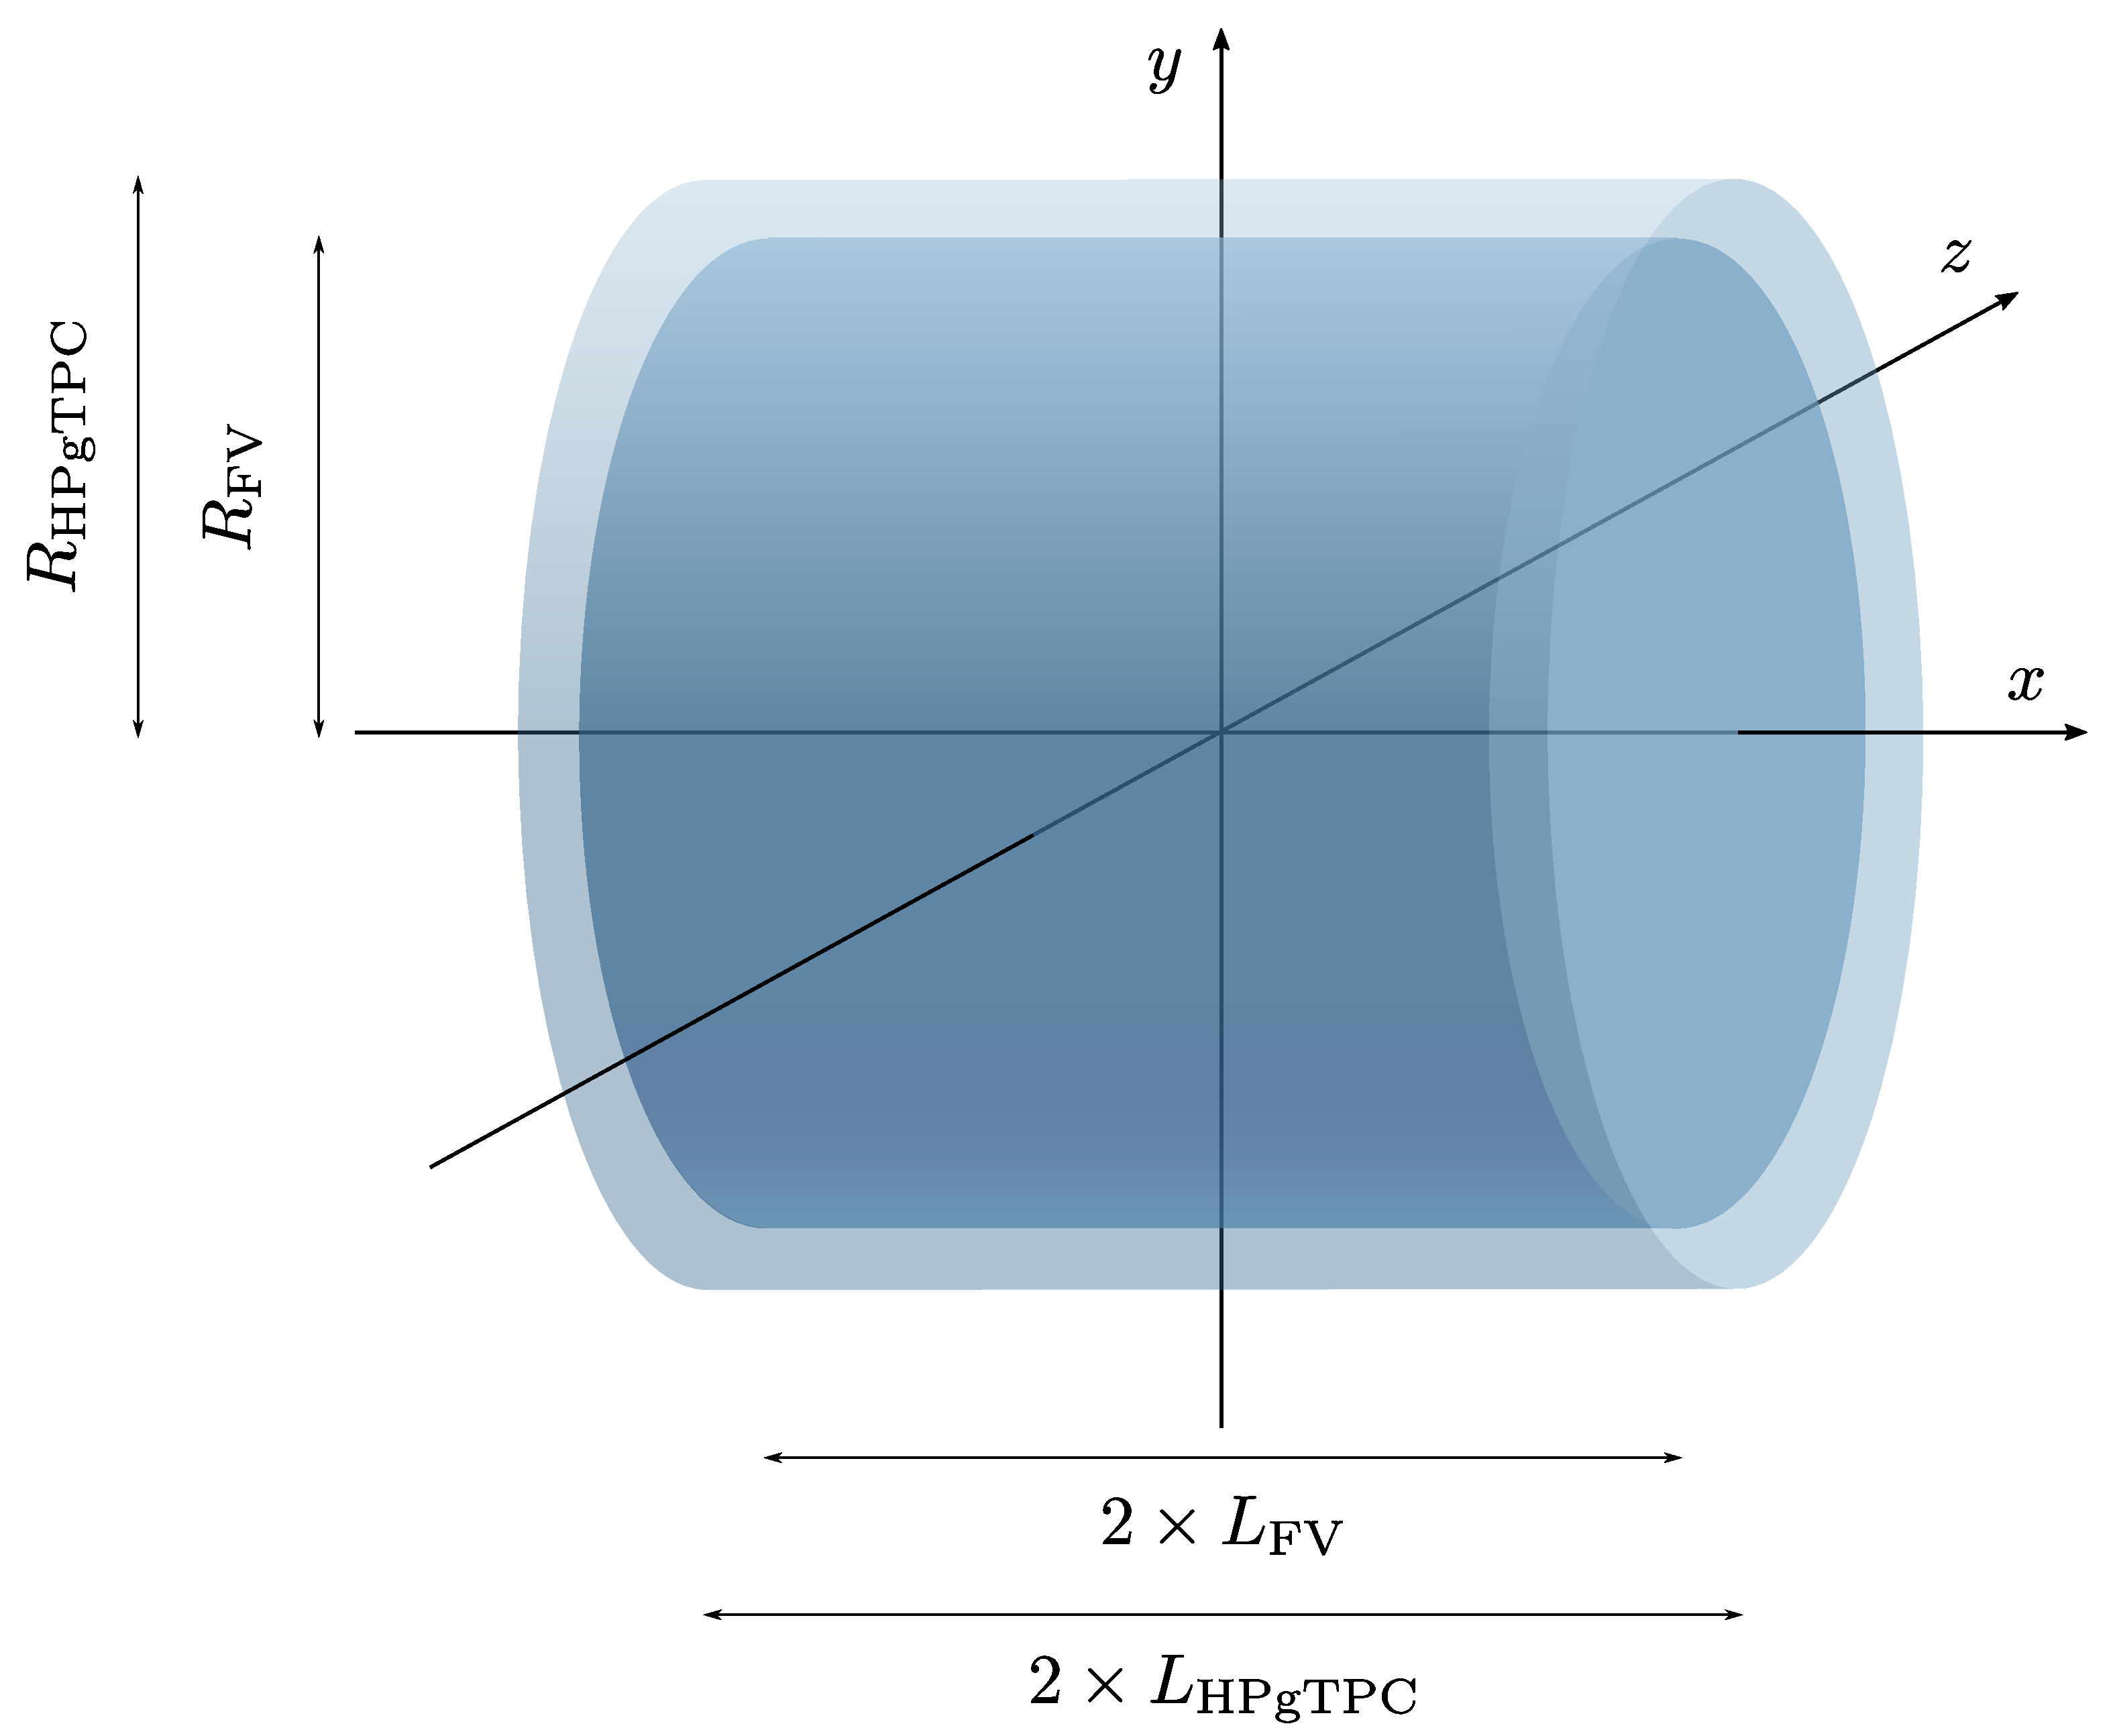
\includegraphics[width=.90\linewidth]{Images/GAr_selection/ndgar_ana_geometry.pdf}
\caption[Schematic diagram of the HPgTPC including the fiducial volume.]{Schematic diagram of the HPgTPC including the fiducial volume (FV). In this case the FV is given by $\Delta L_{\mathrm{FV}} = 30.0 ~ \mathrm{cm}$ and $\Delta R_{\mathrm{FV}} = 30.0 ~ \mathrm{cm}$.}
\label{fig:ndgar_ana_geometry}
\end{figure}

The key to the CC selection is the identification of a primary muon candidate. Typically, this is the longest track in the event. However, sometimes protons and pions leave tracks longer than that of the muon. This is particularly important in the GAr medium, considerably less dense than the LAr. For this reason, the muon identification in ND-GAr relies heavily on the capabilities of the ECal.

The selection strategy proposed combines the information coming from the three main detection systems of ND-GAr: the HPgTPC charge readout, and the ECal and $\mu$ID detectors. It consists of five steps:
\begin{enumerate}
    \item Event contains reconstructed particles.
    \item Select particles with reconstructed negative charge, $q_{\mathrm{reco}} = -1$.
    \item Select particles passing the muon score cut, $\mu_{\mathrm{score}} \geq \mu_{\mathrm{score}}^{\mathrm{cut}}$.
    \item Keep reconstructed particle with the highest momentum, $\mathrm{max}\left[p_{\mathrm{reco}}\right]$.
    \item Check that the remaining particle starts within the FV.
\end{enumerate}
All the events passing these cuts are classified as signal, and the selected particle is regarded as the primary muon candidate.

\begin{figure}[t]
    \centering
    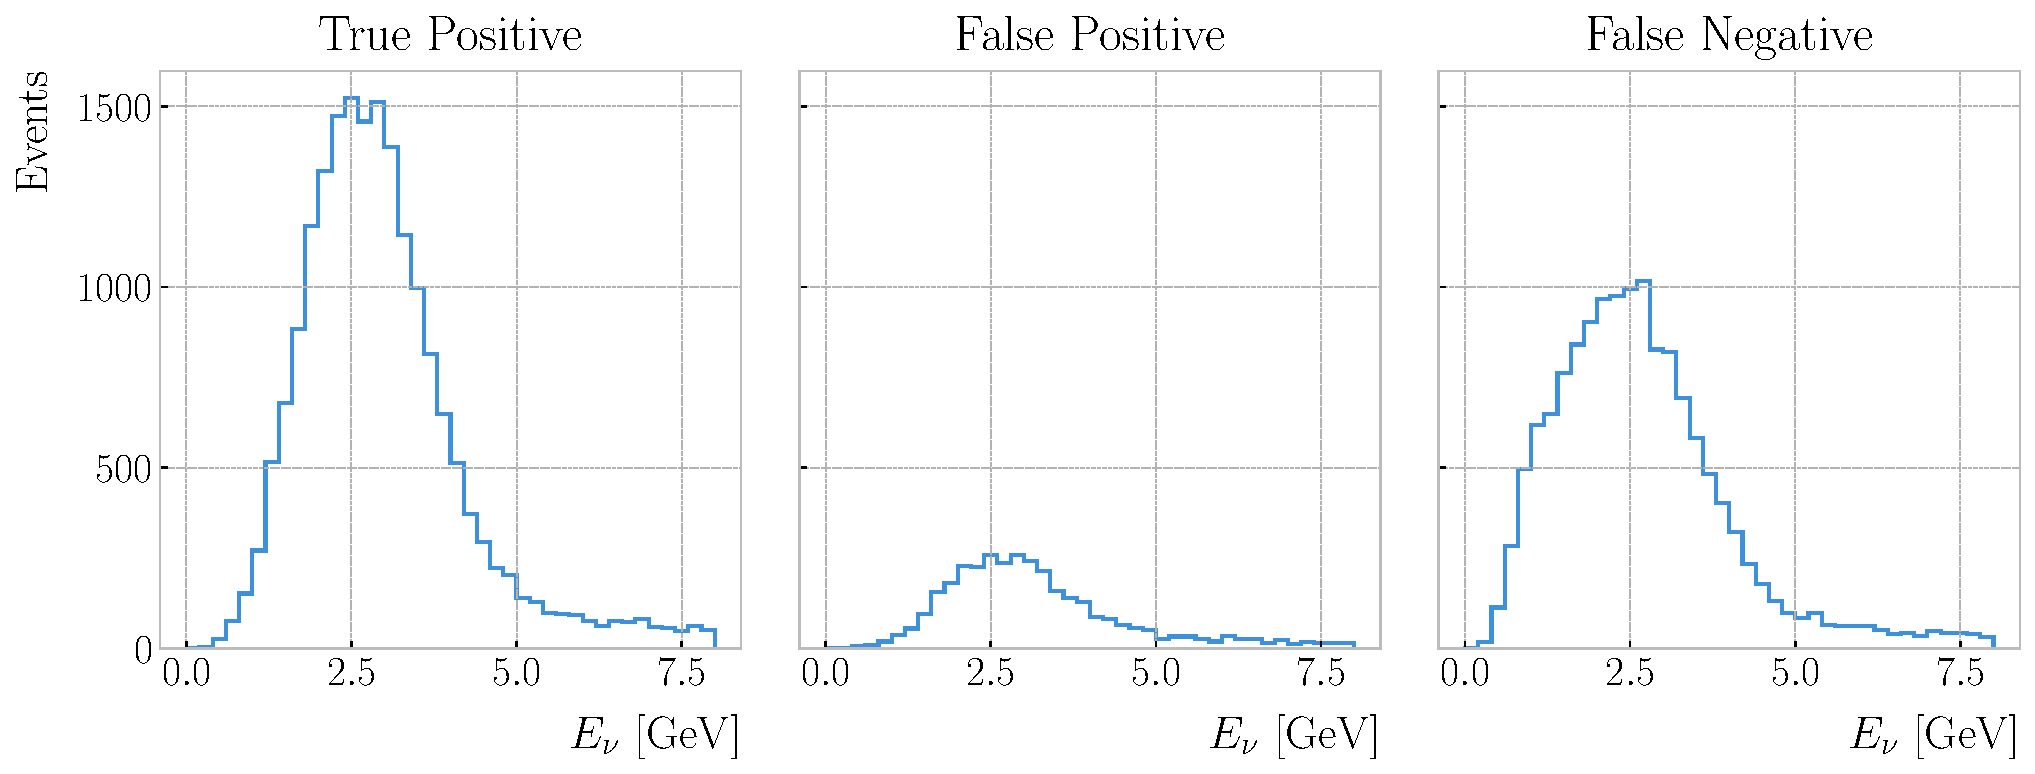
\includegraphics[width=.99\linewidth]{Images/GAr_selection/true_numu_example_spectra_horizontal.pdf}
    \caption[True positive, false positive, and false negative true neutrino energy distributions for a $\nu_{\mu}$ CC selection.]{True positive (left panel), false positive (middle panel), and false negative (right panel) true neutrino energy distributions for the $\nu_{\mu}$ CC selection given by a muon score cut of $\mu_{\mathrm{score}}^{\mathrm{cut}} = 0.75$, and a FV defined as $\Delta L_{\mathrm{FV}} = 30.0 ~ \mathrm{cm}$ and $\Delta R_{\mathrm{FV}} = 30.0 ~ \mathrm{cm}$.}
    \label{fig:numuCC_spectra_example}
\end{figure}

\subsection{Selection optimisation}

I performed an optimisation of this selection, comparing the performance of a number of configurations. For the muon selection, I varied the value of $\mu_{\mathrm{score}}^{\mathrm{cut}}$ from $0.05$ to $0.95$, using a step size of $0.05$. Additionally, to optimise the FV, I systematically explored a number of different parameter configurations, moving within the $10.0-70.0~\mathrm{cm}$ range for $\Delta L_{\mathrm{FV}}$ and $25.0-75.0~\mathrm{cm}$ for $\Delta R_{\mathrm{FV}}$, in increments of $10.0~\mathrm{cm}$ and $5.0~\mathrm{cm}$ respectively.

For each parameter configuration, I extract three different true neutrino energy distributions. These are built combining the results of the selection described previously, which we can refer to as the ``reco'' selection, and a ``true'' selection. The later identifies the true $\nu_{\mu}$ CC events using the GENIE event records, and checks that the true neutrino vertices are contained in the FV.

The first distribution consists of the events passing both selections, i.e., these are the true $\nu_{\mu}$ CC events which pass the ``reco'' selection. The second distribution contains the events passing the ``reco'' selection but failing the ``true'' selection. These are the background events that the selection misidentifies. Finally, the third distribution corresponds to the events picked by the ``true'' selection but not by the ``reco'' one. In other words, these are the true $\nu_{\mu}$ CC events that our selection misses. In analogy to the machine learning jargon, I refer to these distributions as the true positive (TP), false positive (FP), and false negative (FN) spectra, respectively. Figure \ref{fig:numuCC_spectra_example} shows an example of these three distributions for the case $\mu_{\mathrm{score}}^{\mathrm{cut}} = 0.75$, $\Delta L_{\mathrm{FV}} = 30.0 ~ \mathrm{cm}$, and $\Delta R_{\mathrm{FV}} = 30.0 ~ \mathrm{cm}$.

By making different combinations of these distributions one can compute a series of performance metrics. Using the full information from the spectra allows to obtain the scores as a function of the true neutrino energy, whereas the totals can be obtained by integrating the histograms. This way, the efficiency of the selection is given by:
\begin{equation}
    \begin{split}
        \mathrm{Efficiency} &= \frac{\text{Selected true } \nu_{\mu} \text{ CC events}}{\text{Total true } \nu_{\mu} \text{ CC events}}\\
        &= \frac{\mathrm{TP}}{\mathrm{TP}+\mathrm{FN}},
    \end{split}
\end{equation}
while the purity can be written as:
\begin{equation}
    \begin{split}
        \mathrm{Purity} &= \frac{\text{Selected true } \nu_{\mu} \text{ CC events}}{\text{Total selected events}}\\
        &= \frac{\mathrm{TP}}{\mathrm{TP}+\mathrm{FP}}.
    \end{split}
\end{equation}

Another scoring metric typically used when quantifying the performance of a selection is the significance. It is defined as:
\begin{equation}
    \mathrm{Significance} = \frac{S}{\sqrt{S+B}} = \frac{\mathrm{TP}}{\sqrt{\mathrm{TP} + \mathrm{FP}}}.
\end{equation}
The significance measures the relative size of the true signal within the selection, $S=\mathrm{TP}$ with respect to one standard deviation of the counting experiment. Assuming Poisson statistics, the variance is equal to the number of observations, and therefore the standard deviation equals to $\sqrt{N}=\sqrt{S+B}=\sqrt{\mathrm{TP} + \mathrm{FP}}$. I use this metric to 

\begin{figure}[t]
    \centering
    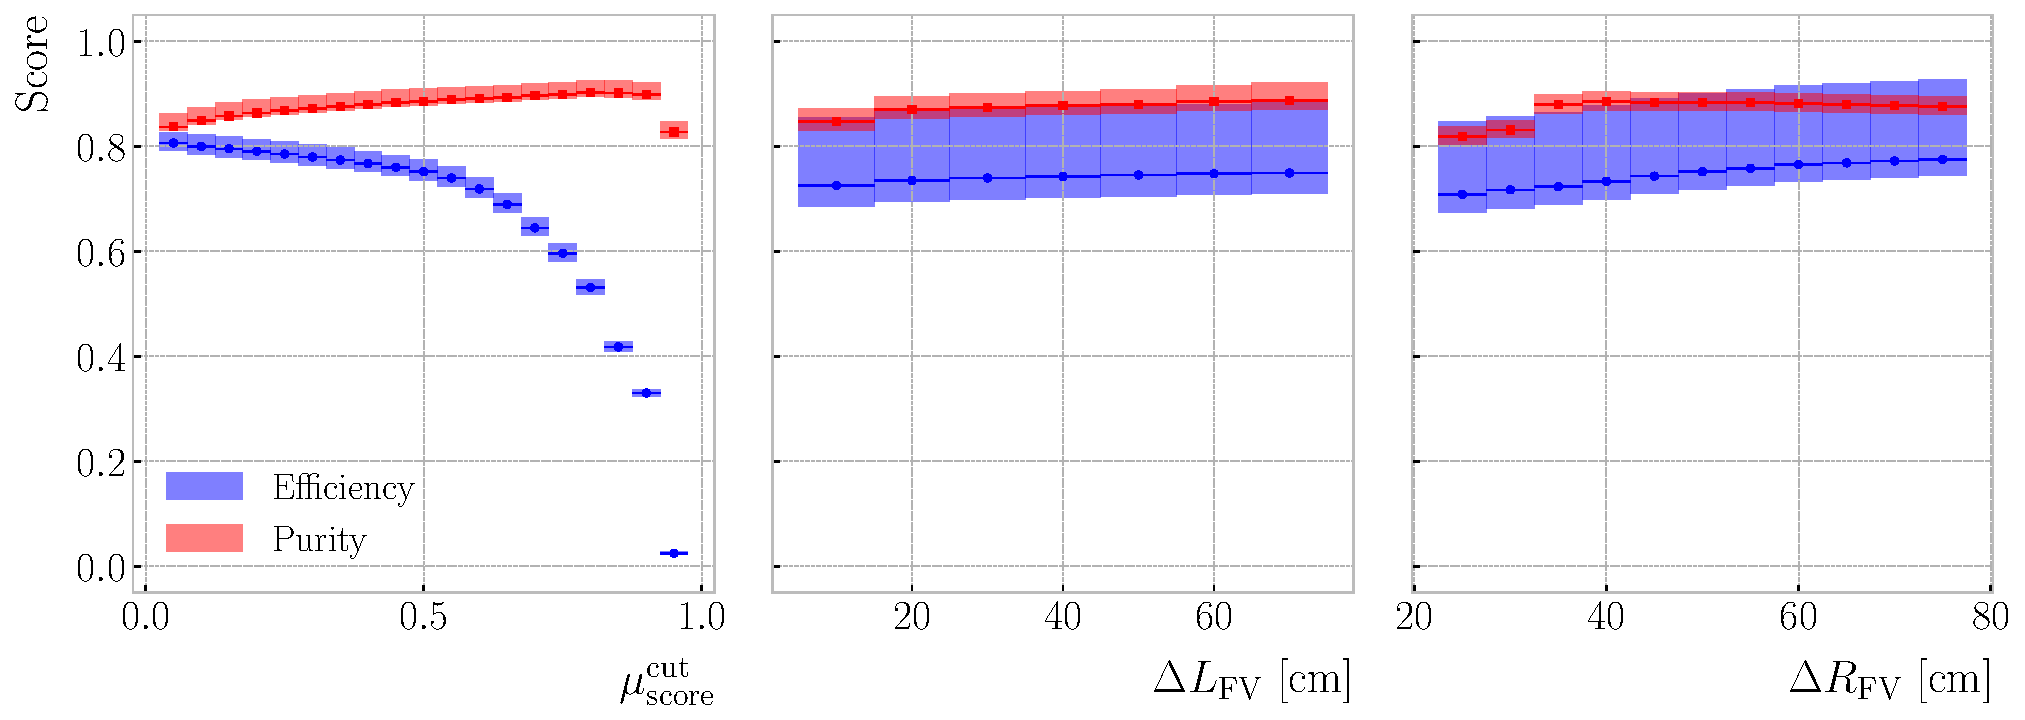
\includegraphics[width=.99\linewidth]{Images/GAr_selection/efficiency_and_purity_error_boxes.pdf}
    \caption[Efficiency and purity for the $\nu_{\mu}$ CC selection as a function of the different cuts.]{Efficiency (blue) and purity (red) for the $\nu_{\mu}$ CC selection as a function of the muon score cut (left panel), FV half-length cut (middle panel), and radial cut (right panel). The height of the boxes represents the IQR of the conditional distributions, whereas the horizontal line corresponds to the median.}
    \label{fig:numuCC_metrics_opt}
\end{figure}

\begin{figure}[t]
    \centering
    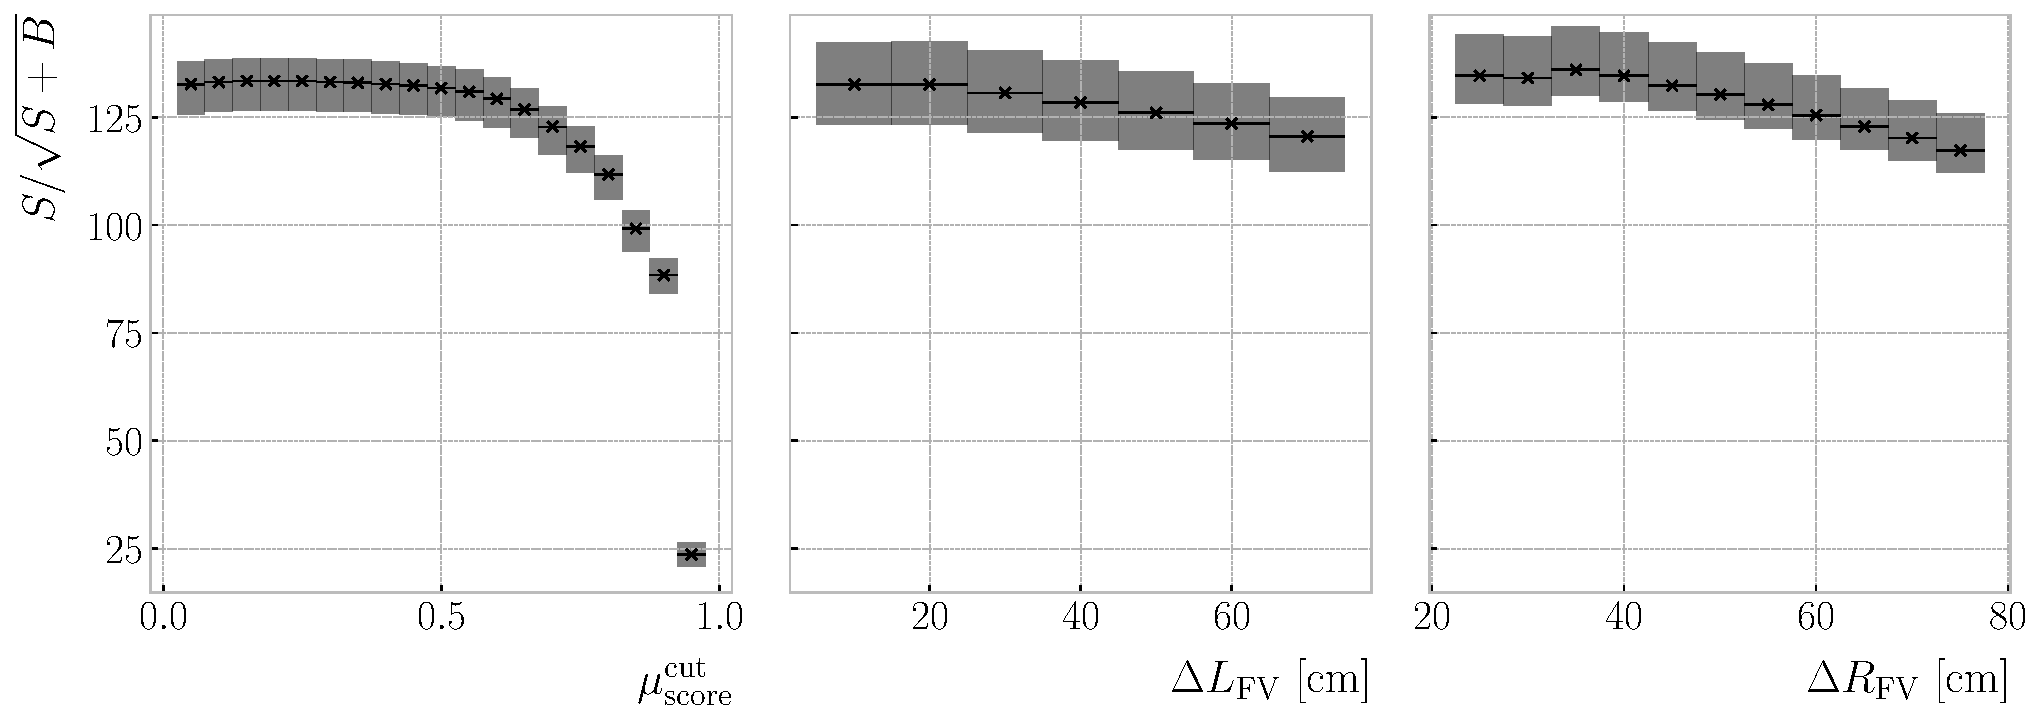
\includegraphics[width=.99\linewidth]{Images/GAr_selection/significance_error_boxes.pdf}
    \caption[Significance for the $\nu_{\mu}$ CC selection as a function of the different cuts.]{Significance for the $\nu_{\mu}$ CC selection as a function of the muon score cut (left panel), FV half-length cut (middle panel), and radial cut (right panel). The height of the boxes represents the IQR of the conditional distributions, whereas the horizontal line corresponds to the median.}
    \label{fig:numuCC_significance_opt}
\end{figure}

Figure \ref{fig:numuCC_metrics_opt} shows the change in efficiency (blue) and purity (red) of the $\nu_{\mu}$ CC selection as a function of the different cuts. From left to right, I vary $\mu_{\mathrm{score}}^{\mathrm{cut}}$, $\Delta L_{\mathrm{FV}}$, and $\Delta R_{\mathrm{FV}}$. For each value of the cuts, I compute the median and IQR (represented by the horizontal lines and the heights of the boxes, respectively) of the corresponding conditional distributions of efficiency and purity. This representation is useful to get an idea of the general trend the scores follow with the cuts, as well as the spread. It is clear that the muon score cut has the biggest impact on the efficiency, which ranges between $0.05$ to $0.80$, whereas the purity remains stable with values around $0.85$.

\begin{figure}[t]
    \centering
    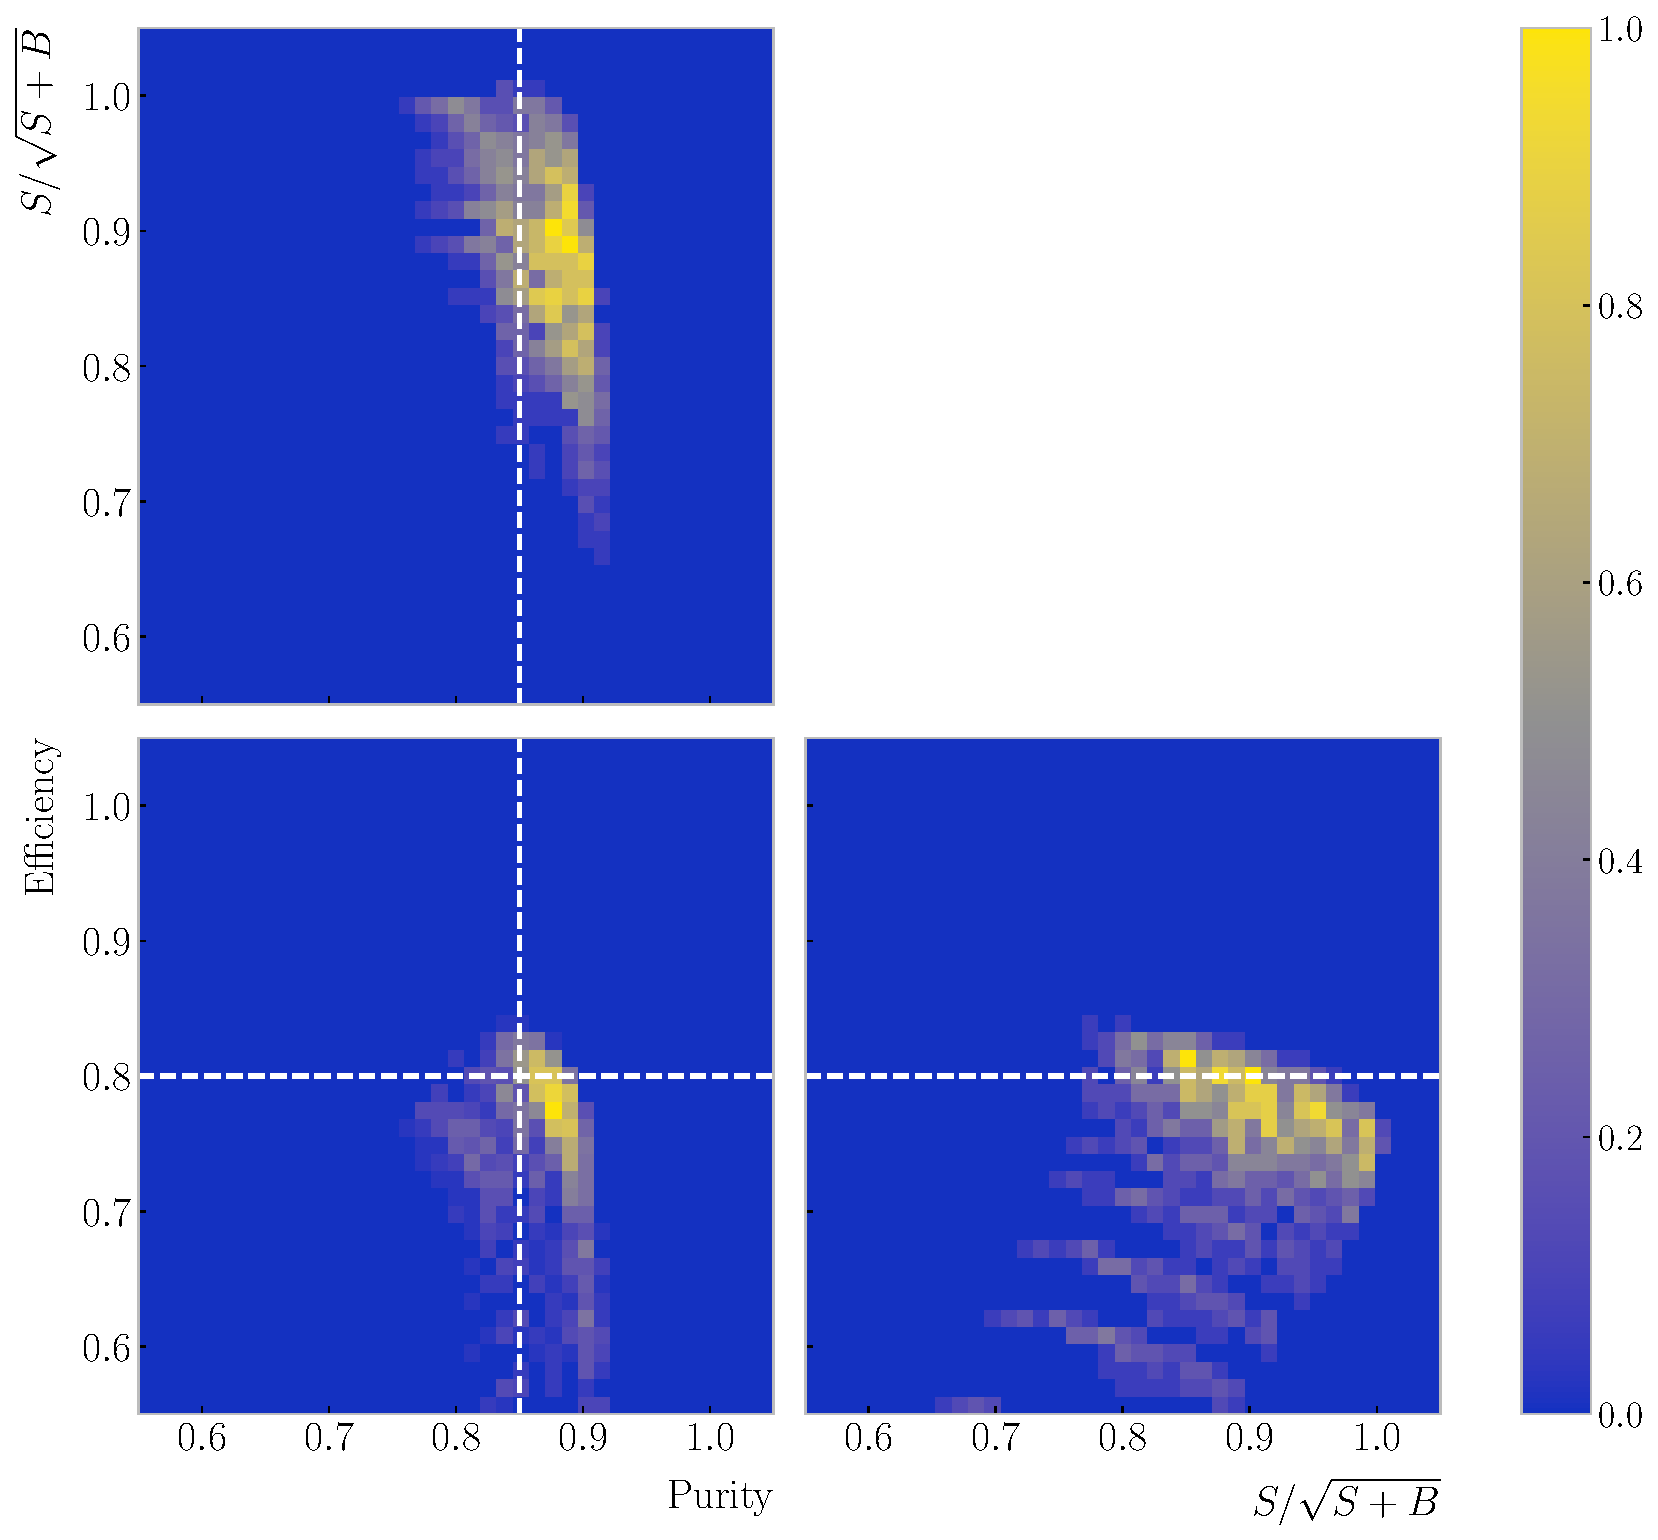
\includegraphics[width=.95\linewidth]{Images/GAr_selection/numuCC_metric_heatmap.pdf}
    \caption{Normalised 2D distributions of efficiency, purity and significance for the $\nu_{\mu}$ CC selection. The $S/\sqrt{S+B}$ is normalised to the highest value achieved. The vertical dashed line indicates a purity value of $0.85$, whereas the horizontal one corresponds to an efficiency of $0.80$.}
    \label{fig:numuCC_metric_heat}
\end{figure}

A similar depiction of the significance can be found in Fig. \ref{fig:numuCC_significance_opt}. In this case, one can see that the $S/\sqrt{S+B}$ decreases as the cuts grow tighter. However, there are hints of local maxima at intermediate values.

Selecting the cut configuration with the highest significance, $147 \pm 11$ for the parameter values explored here, results in an efficiency and purity of $0.754 \pm 0.006$ and $0.833 \pm 0.007$, respectively. Figure \ref{fig:numuCC_metric_heat} shows the 2D distributions resulting when combining pairs of efficiency, purity and significance, obtained for the cut configurations explored. The significance is normalised to the highest value obtained in the parameter scan. Looking at this, it is clear that a selection with highest efficiency and purity can be achieved, maintaining a similar significance level.

\begin{figure}[t]
	\centering
	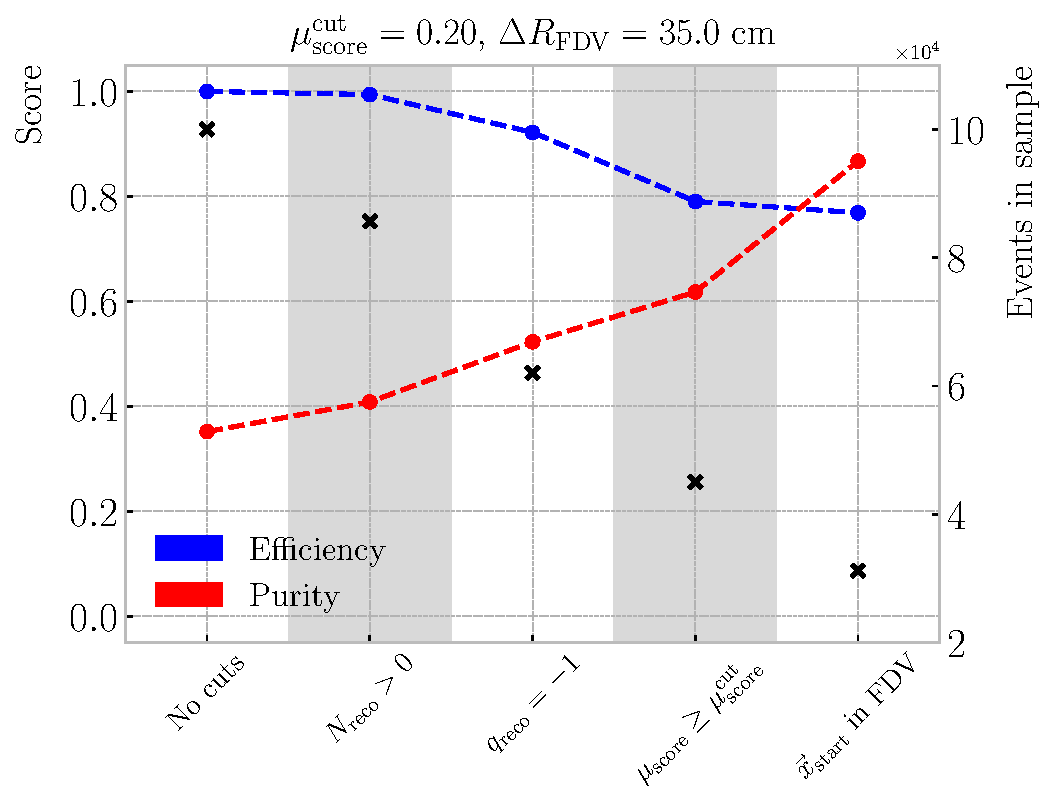
\includegraphics[width=.90\linewidth]{Images/GAr_selection/numu_cc_selection_steps.pdf}
	\caption[Cumulative efficiency and purity for the $\nu_{\mu}$ CC selection.]{Cumulative efficiency (blue) and purity (red) of the $\nu_{\mu}$ CC selection. The secondary axis indicates the number of events in the sample after each cut (black crosses).}
	\label{fig:numuCC_selection_steps}
\end{figure}

\begin{table}[h!]
	\caption[Step-by-step $\nu_{\mu}$ CC selection cuts and cumulative passing rates.]{Step-by-step $\nu_{\mu}$ CC selection cuts and cumulative passing rates. Relative passing rates are indicated in parentheses.}
	\begin{center}
		\begin{small}
			\begin{tabular}{c|ccc}
                Cut \# & Selection cut                       & Events & Passing rates          \\[2mm] \hline
                \rule{0pt}{1.1\normalbaselineskip}0      & Total number of events (No cuts)    & 100000 & $100.00\% ~(100.00\%)$ \\[2mm]
                1      & At least one reconstructed particle                              & 85680  & $85.68 \% ~(85.68 \%)$ \\[2mm]
                2      & Negatively charged particles only                                & 62054  & $62.05\% ~(72.43\%)$   \\[2mm]
                3      & $\mu_{\mathrm{score}} \geq \mu_{\mathrm{score}}^{\mathrm{cut}}$  & 46585  & $46.59\% ~(75.07\%)$   \\[2mm]
                4      & Candidate $\vec{x}_{\mathrm{start}}$ in FV                       & 31834  & $31.83\% ~(68.34\%)$  
                \end{tabular}
		\end{small}
	\end{center}
	\label{tab:numuCC_selection}
\end{table}

Therefore, to get a more refined selection, I first select the configurations with a purity and an efficiency higher than $0.85$ and $0.80$, respectively. After that, I select the tuple of cuts yielding the highest significance. The resulting value for the muon score cut is $\mu_{\mathrm{score}}^{\mathrm{cut}} = 0.10$, and the FV is given by $\Delta L_{\mathrm{FV}} = 30.0~\mathrm{cm}$ and $\Delta R_{\mathrm{FV}} = 50.0~\mathrm{cm}$. With these, one obtains a total efficiency of $0.800 \pm 0.007$ and purity of $0.851 \pm 0.008$, with a significance of $138 \pm 11$. Hereafter, I use this optimised selection cuts, unless specified otherwise.

A summary of the selection can be found in Tab. \ref{tab:numuCC_selection}. It shows the number of events in the selected sample after each selection cut, as well as the absolute and relative passing rates. Figure \ref{fig:numuCC_selection_steps} shows the overall efficiencies (blue) and purities (red) after each cut in the event selection is applied. As expected, the efficiency drops while the purity increases with the successive cuts.

Notice how, out of the cuts prior to the FV constraint, the sign selection produces the highest increase in purity. This is one of the advantages of having a magnetised TPC, and can also be used for a $\bar{\nu}_{\mu}$ CC selection when running in RHC mode.

\begin{figure}[t]
	\centering
	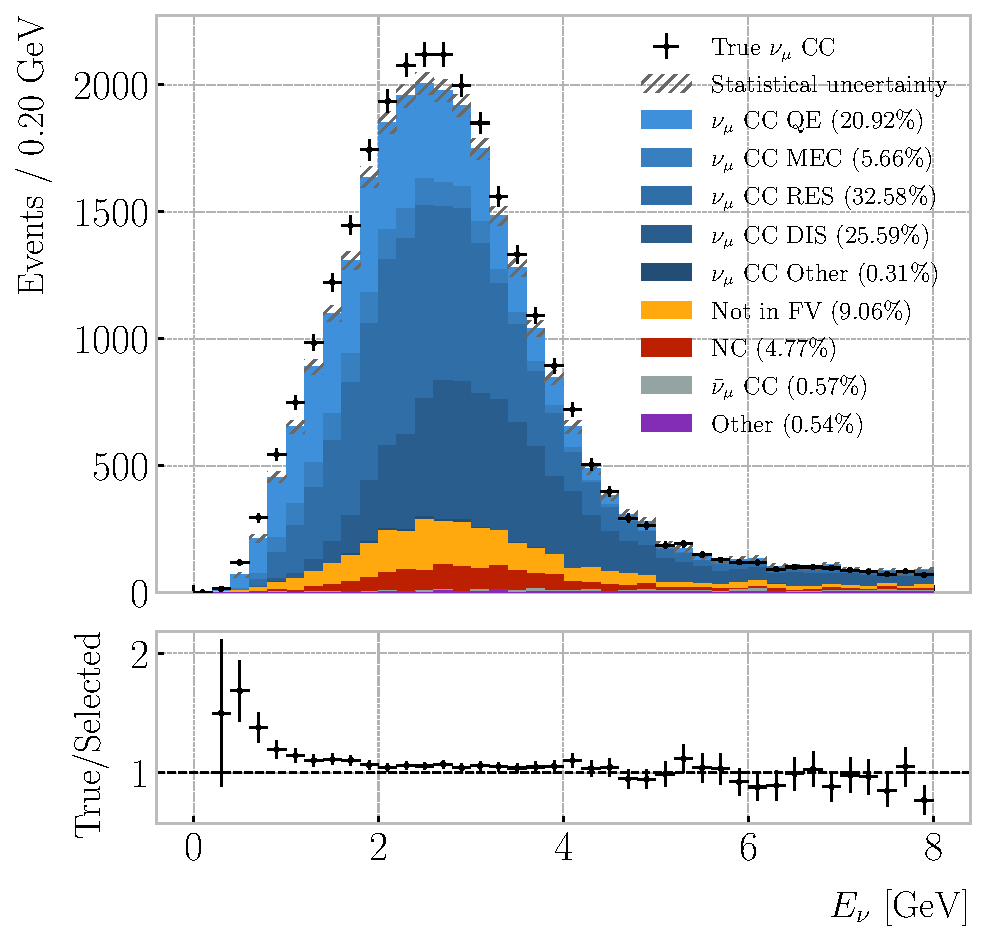
\includegraphics[width=.80\linewidth]{Images/GAr_selection/numuCC_selection_true_energy.pdf}
	\caption[True neutrino energy spectra for the $\nu_{\mu}$ CC selection.]{True neutrino energy spectra for the $\nu_{\mu}$ CC selection. The selected events correspond to the coloured stacked histogram, broken down by signal and background subcategories. The statistical uncertainty is drawn in hatched gray. The true distribution is also shown with the black data points. The bottom panel shows the ratio between the number of true and selected $\nu_{\mu}$ CC events per bin.}
	\label{fig:numuCC_selection_true_enu}
\end{figure}

\begin{figure}[t]
	\centering
	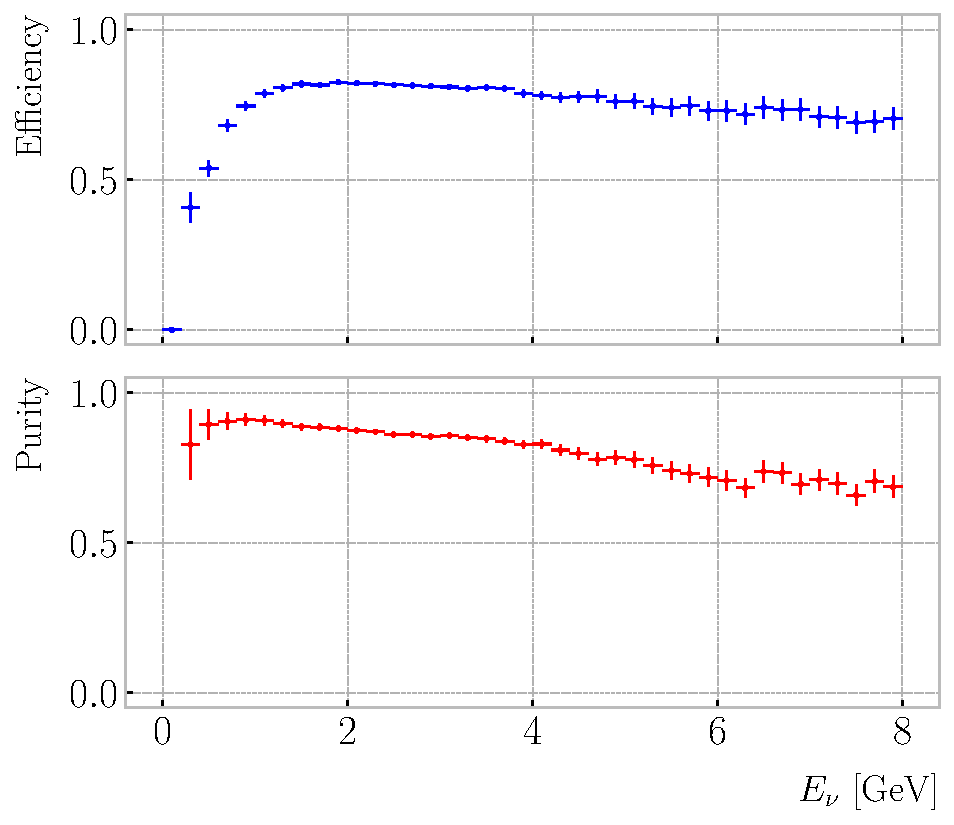
\includegraphics[width=.99\linewidth]{Images/GAr_selection/numuCC_selection_true_energy_performance.pdf}
	\caption[True neutrino energy spectra for the $\nu_{\mu}$ CC selection.]{Left panel: efficiency (top panel) and purity (bottom panel) for the $\nu_{\mu}$ CC selection as a function of the true neutrino energy. Right panel: significance for the $\nu_{\mu}$ CC selection as a function of the true neutrino energy}
	\label{fig:numuCC_selection_true_enu_performance}
\end{figure}

\subsection{Selection performance}

Using the stored spectra discussed above, the true neutrino energy distribution for the selected events can be recovered doing $\mathrm{TP}+\mathrm{FP}$. Similarly, the combination $\mathrm{TP}+\mathrm{FN}$ gives the true spectrum. Figure \ref{fig:numuCC_selection_true_enu} shows the true (black data points) and selected (coloured stacked histogram) $E_{\nu}$ distributions for the optimised $\nu_{\mu}$ CC selection. The colours in the selected spectrum indicate the different signal categories and backgrounds, with the overall statistical uncertainty represented by the gray hatched mess. The ratio between the true and selected events is also shown. One can see that it sits around $1$ for most of the energy range. However, for energies $\leq 1~\mathrm{GeV}$ there is a significant deficit of selected events.

\begin{figure}[t]
	\centering
	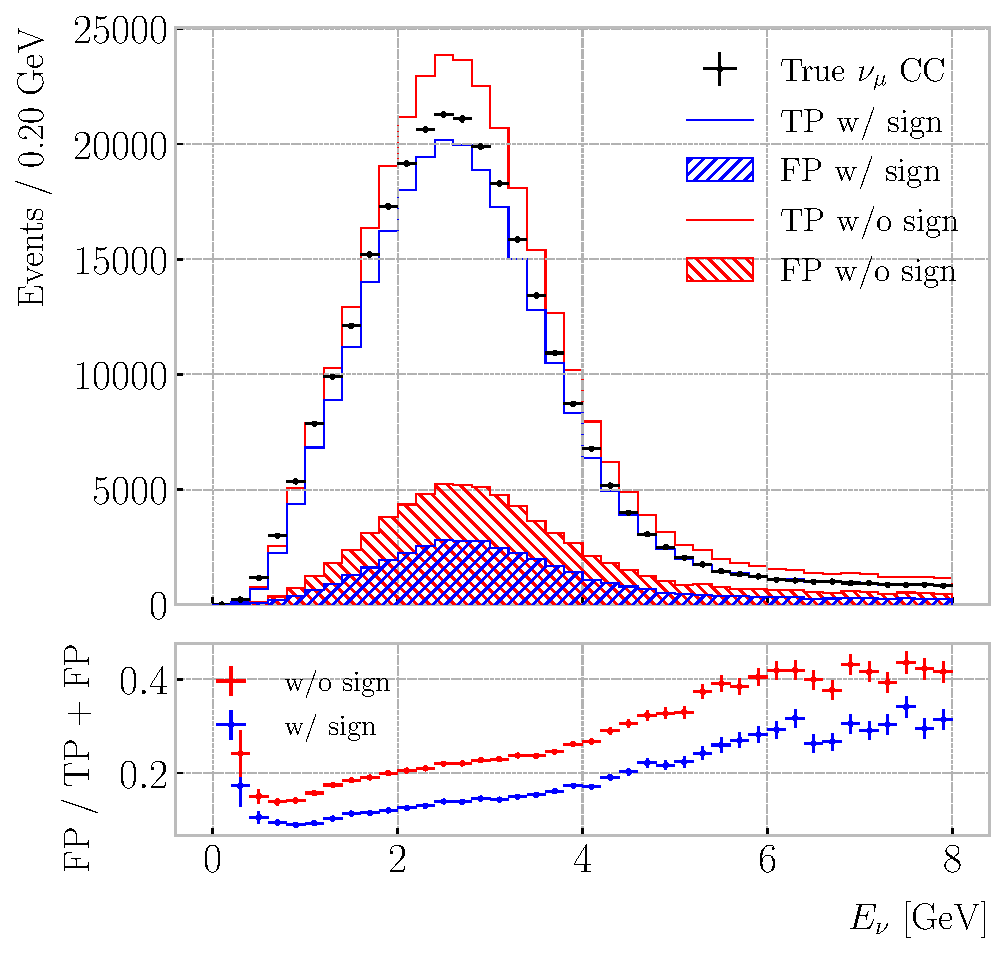
\includegraphics[width=.80\linewidth]{Images/GAr_selection/numuCC_selection_true_energy_sign_comp.pdf}
	\caption{True neutrino energy spectra for the $\nu_{\mu}$ CC selection with (blue) and without (red) sign selection. The selected events are broken down by true positives (signal) and false positives (background). The true distribution is also shown (black data points). The bottom panel shows the ratios between the number of false positives and total selected events per bin.}
	\label{fig:numuCC_sign_selection}
\end{figure}

These spectra also allow to compute the efficiency and purity of the selection as a function of the true neutrino energy, as shown in Fig. \ref{fig:numuCC_selection_true_enu_performance} (left panel). As it could be expected from the previous ratio plot, the efficiency is low at low neutrino energies. Nonetheless, it raises quickly with the energy, until it stabilises around a value of $0.80$. Looking at the purity, one may notice that, although it starts at around $0.90$, there is a significant decrease towards the high end of the spectrum. Figure \ref{fig:numuCC_selection_true_enu_performance} (right panel) also shows the significance as a function of the energy. In this case, the highest $S/\sqrt{S+B}$ is achieved around the energies where the spectrum peaks.

A variation of the $\nu_{\mu}$ CC selection one can try is to apply it without the reconstructed charge cut. Figure \ref{fig:numuCC_sign_selection} (top panel) shows the $E_{\nu}$ distributions corresponding to the selection with (blue stacked histogram) and without (red stacked histogram) the sign selection. In the former case, the out of FV contamination amounts to $9.06\%$ of the total, while the NC contamination results $4.77\%$ and the wrong-sign contamination $0.57\%$. For the later, these backgrounds account for the $10.01\%$, $10.82\%$, and $2.18\%$ of the selected events, respectively. As expected, removing the positive particles does not change the FV-related effects noticeably. However, the sign selection proves its worth in the rejection of $\bar{\nu}_{\mu}$ CC events, which drop almost by one order of magnitude. Additionally, the charge selection cuts the NC events in half, as it reduces the chances of misidentifying a positively charged hadron for a muon.

\begin{figure}[t]
	\centering
	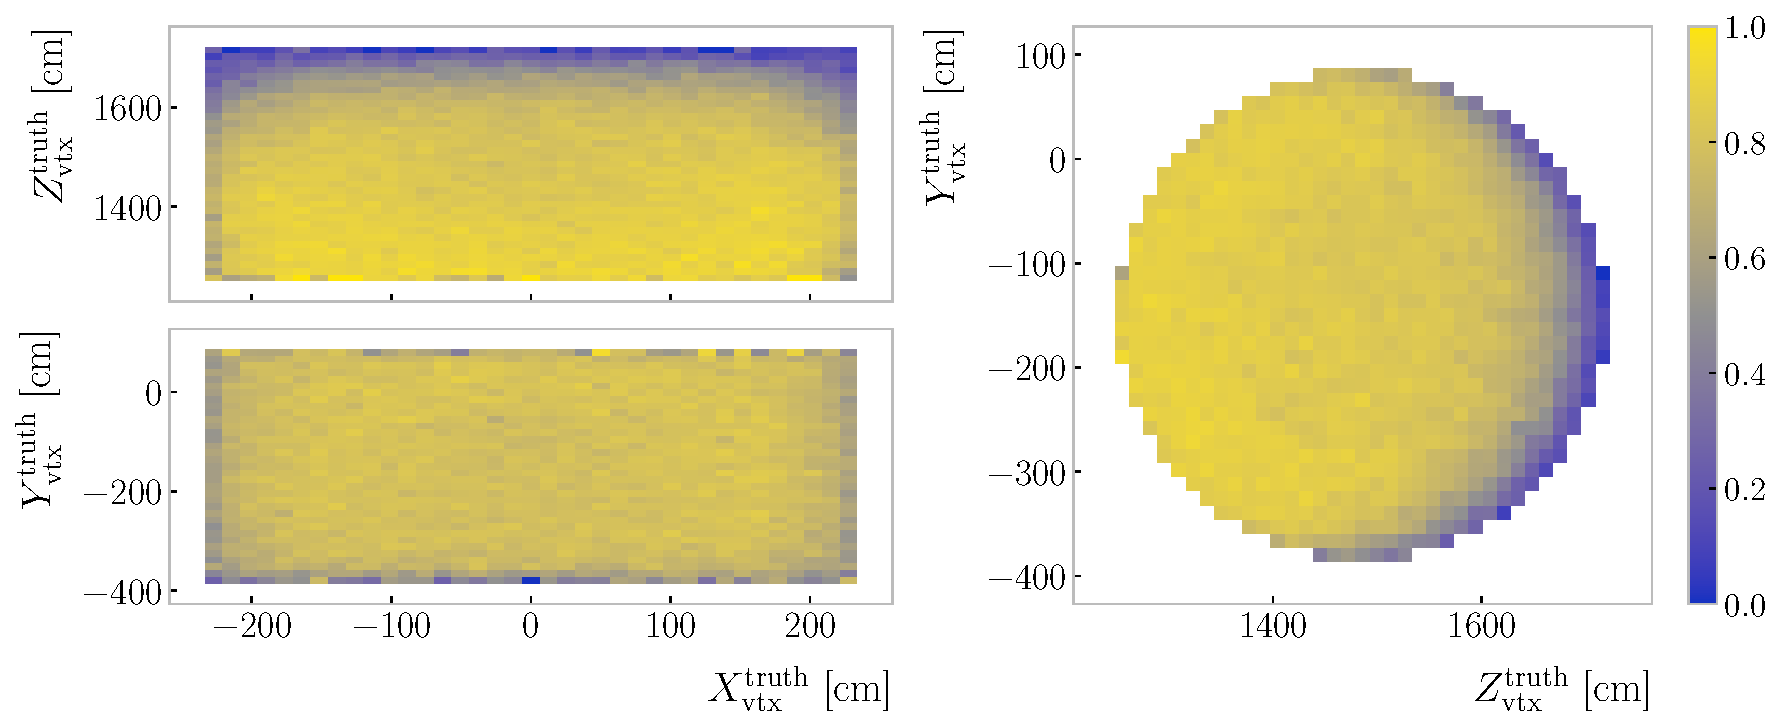
\includegraphics[width=.99\linewidth]{Images/GAr_selection/numuCC_selection_true_vertex_performance.pdf}
	\caption{Efficiency 2D distributions for the $\nu_{\mu}$ CC selection given the true position of the interaction vertex.}
	\label{fig:numuCC_vertex_efficiency}
\end{figure}

As an additional check, I explored how the performance of the $\nu_{\mu}$ CC selection depends on the position of the neutrino interaction within the HPgTPC. Maps of the selection efficiency for the $X,Z$ (top left panel), $X,Y$ (bottom left panel), and $Z,Y$ (right panel) true vertex position pairs are given in Fig. \ref{fig:numuCC_vertex_efficiency}. It can be seen that the efficiency remains stable along the drift direction, only slightly degrading close to the edges of the FV. Regarding the radial direction, it is clear that an important number of events with high $Z^{\mathrm{truth}}_{\mathrm{vtx}}$ are not being selected. Intuitively, the muons arising from these interactions will leave short tracks. As their directions are typically aligned with the beam direction, they enter the ECal shortly after production. This is likely to affect the tracking, and therefore their identification. As a result, the regions with the lowest efficiency are the downstream corners of the HPgTPC, i.e. the areas with high $|X^{\mathrm{truth}}_{\mathrm{vtx}}|$ and $Z^{\mathrm{truth}}_{\mathrm{vtx}}$.

\begin{comment}
\begin{figure}[t]
	\begin{subfigure}{0.5\textwidth}
		\centering
		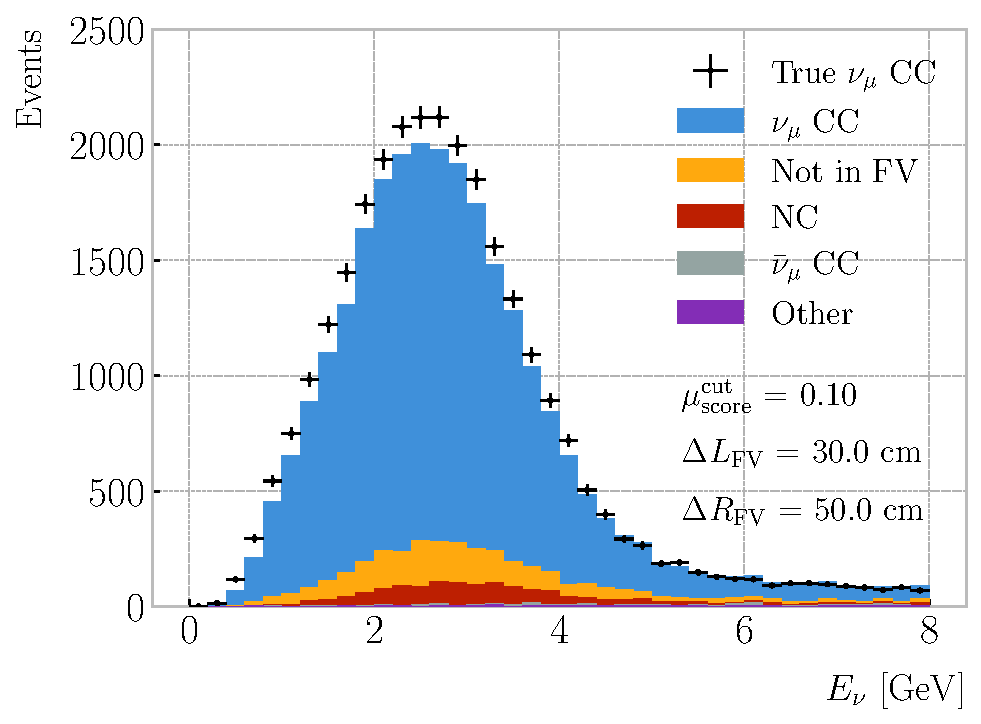
\includegraphics[width=.99\linewidth]{Images/GAr_selection/nu_energy_with_breakdown.pdf}
	\end{subfigure}
	\begin{subfigure}{0.5\textwidth}
		\centering
		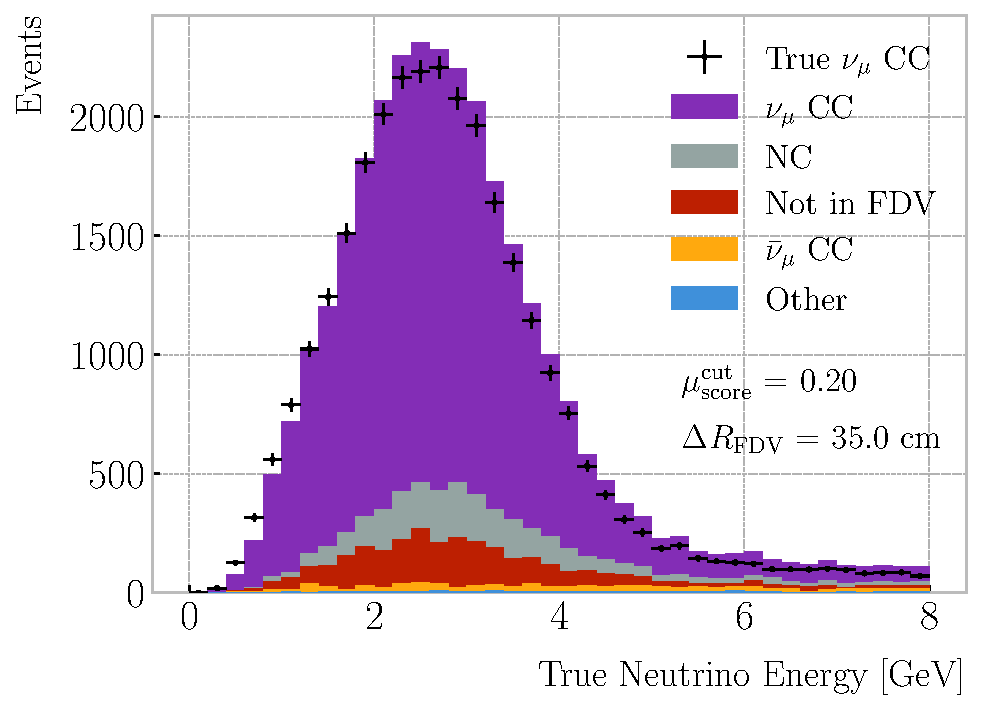
\includegraphics[width=.99\linewidth]{Images/GAr_selection/nu_energy_with_breakdown_no_sign.pdf}
	\end{subfigure}
	\caption[True neutrino energy spectra for the $\nu_{\mu}$ CC selection with and without sign selection.]{True neutrino energy spectra for the $\nu_{\mu}$ CC selection with (left panel) and without (right panel) sign selection. The selected events are broken down by signal or background category. The true distribution is also shown (black data points).}
	\label{fig:numuCC_sign_selection}
\end{figure}
\end{comment}

\begin{figure}[t]
    \centering
    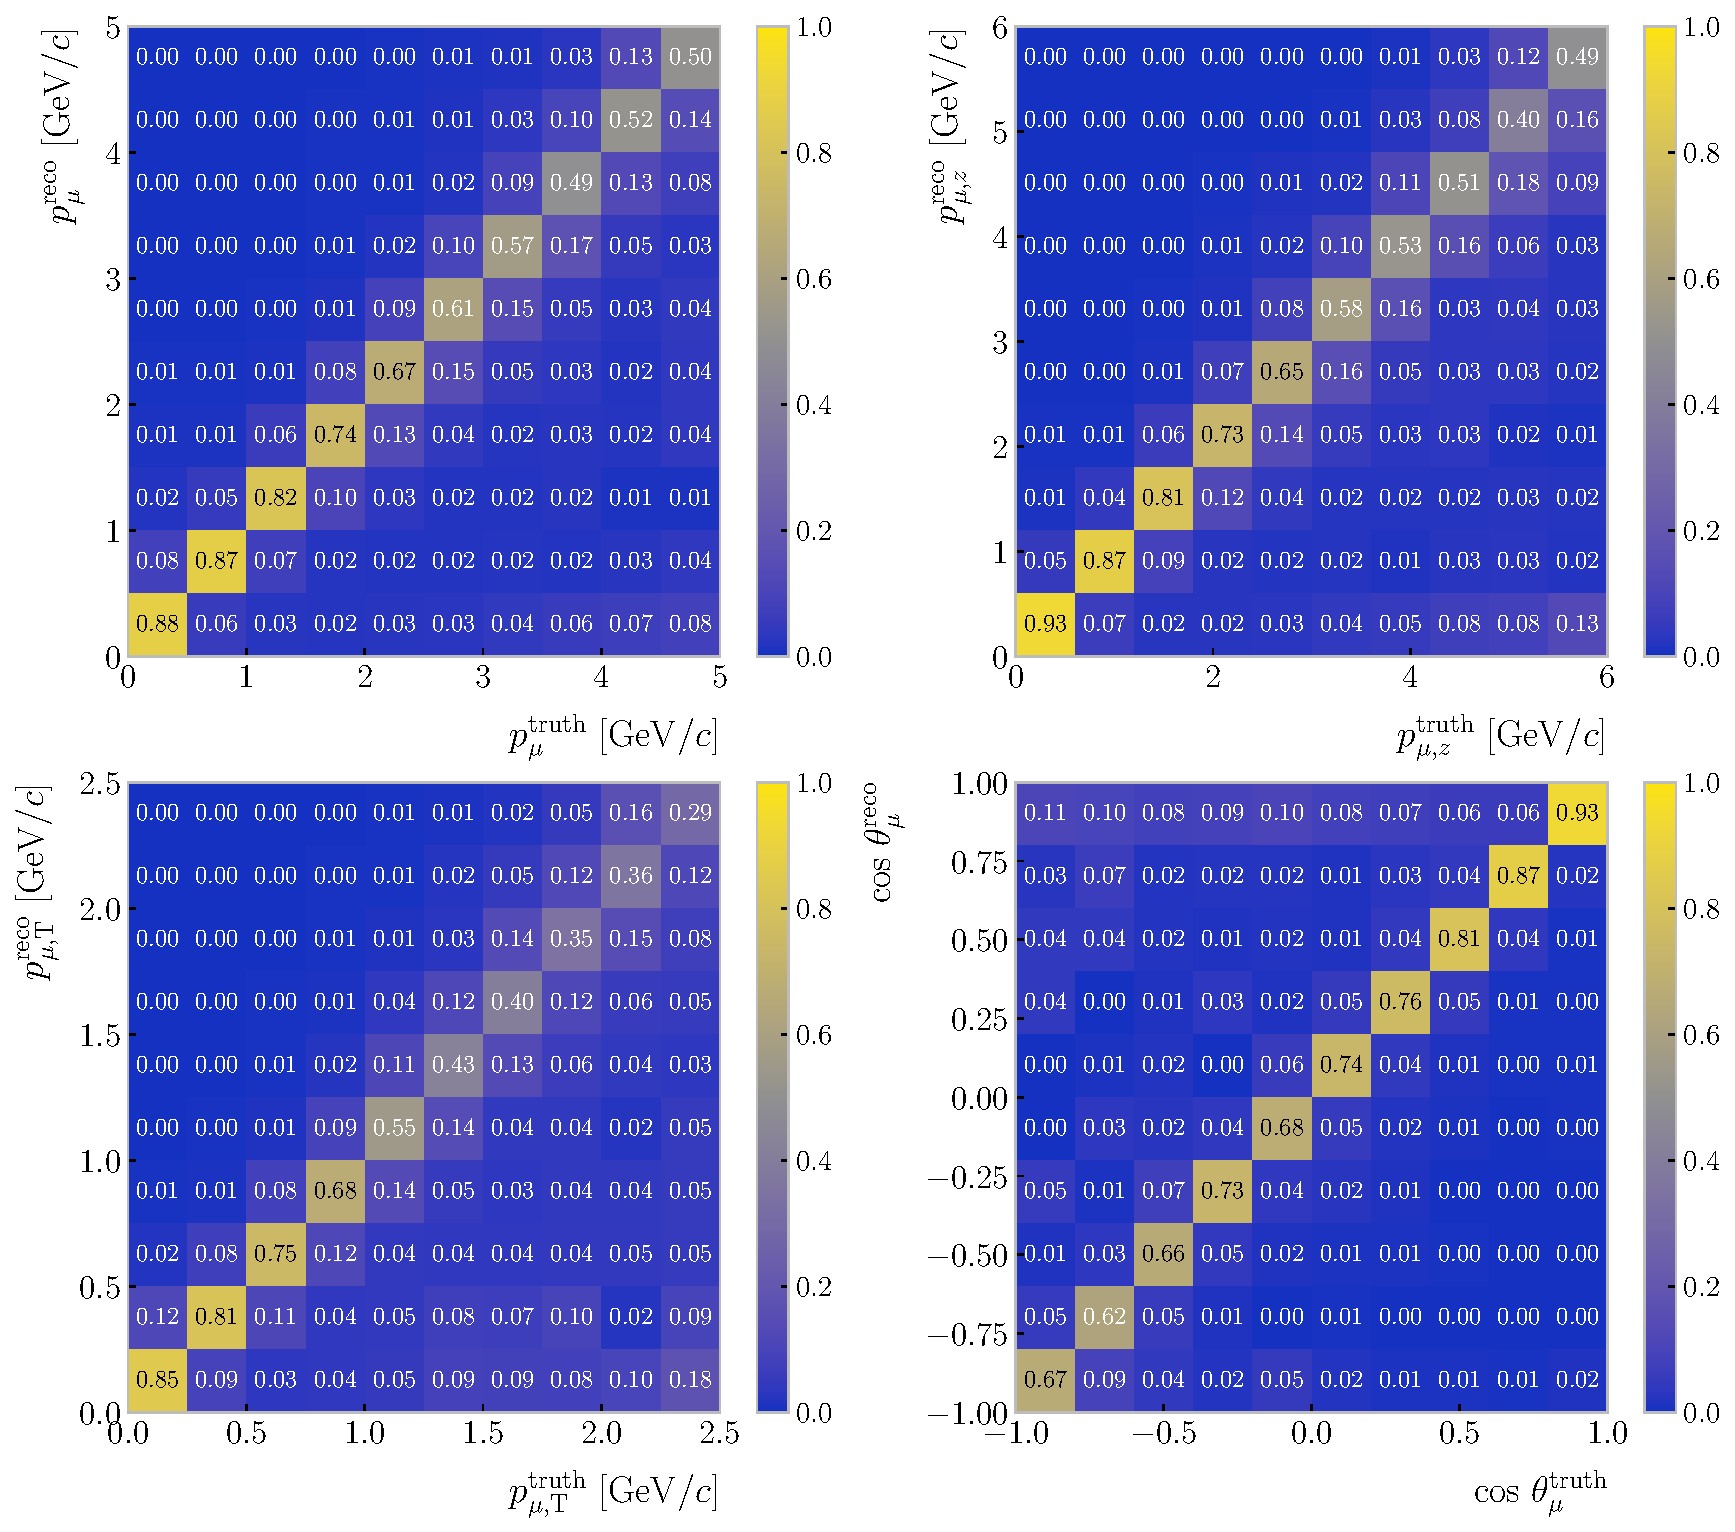
\includegraphics[width=.99\linewidth]{Images/GAr_selection/numuCC_muon_kinematic_comp.pdf}
    \caption{Distributions for the reconstructed versus truth generated primary muon momentum (top left panel), longitudinal momentum (top right panel), transverse momentum (bottom left panel), and beam angle (bottom right panel). The reconstructed values correspond to the selected primary muon candidate, whereas the truth values come from the true primary muon in the event.}
    \label{fig:numuCC_muon_kinematic_comp}
\end{figure}

\subsection{Primary muon kinematics}

This $\nu_{\mu}$ CC selection relies on the identification of the a primary muon, meaning that for each selected event a particle is picked out as the muon candidate. It is because of this that one can study the kinematics of these selected primary muons.

Figure \ref{fig:numuCC_muon_kinematic_comp} shows a comparison between some of the reconstructed and truth primary muon kinematic variables. From top to bottom, left to right, we have muon momentum, longitudinal momentum, transverse momentum and beam angle. The histograms are column-normalised, and so the diagonal entries give an idea of the resolution for the different variables. The match between truth and reconstructed values can only be done for the selected true $\nu_{\mu}$ CC events, as the others do not have a primary muon. However, for this comparison I do not require the events to start inside the FV.

\begin{figure}[t]
	\centering
	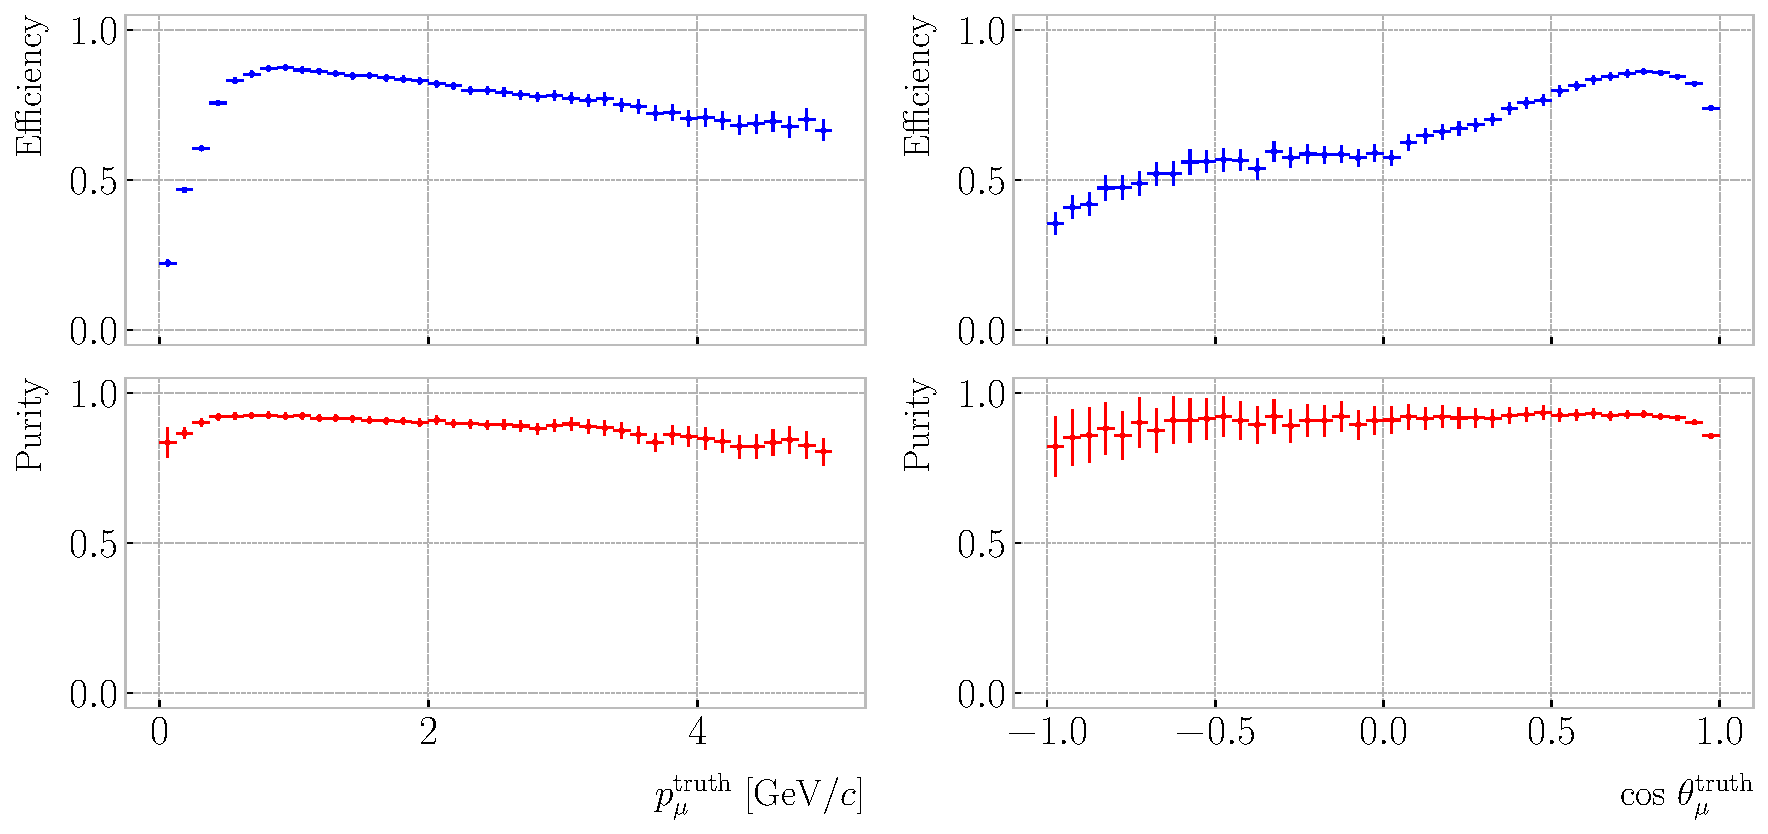
\includegraphics[width=.99\linewidth]{Images/GAr_selection/numuCC_selection_true_kinematics_performance.pdf}
	\caption[Efficiency and purity of the $\nu_{\mu}$ CC selection as a function of the primary muon true momentum and beam angle.]{Efficiency (blue) and purity (red) of the $\nu_{\mu}$ CC selection as a function of the primary muon true momentum (left panel) and beam angle (right panel).}
	\label{fig:numuCC_muon_kinematics}
\end{figure}

Notice that, for the reconstructed values, the variables do not necessarily come from a reconstructed particle that matches the true primary muon. In other words, sometimes, even though the event was correctly identified, the primary muon may have been confused with another particle. That means that in these distributions include both reconstruction and selection deficiencies.

\begin{figure}[p!]
    \centering
    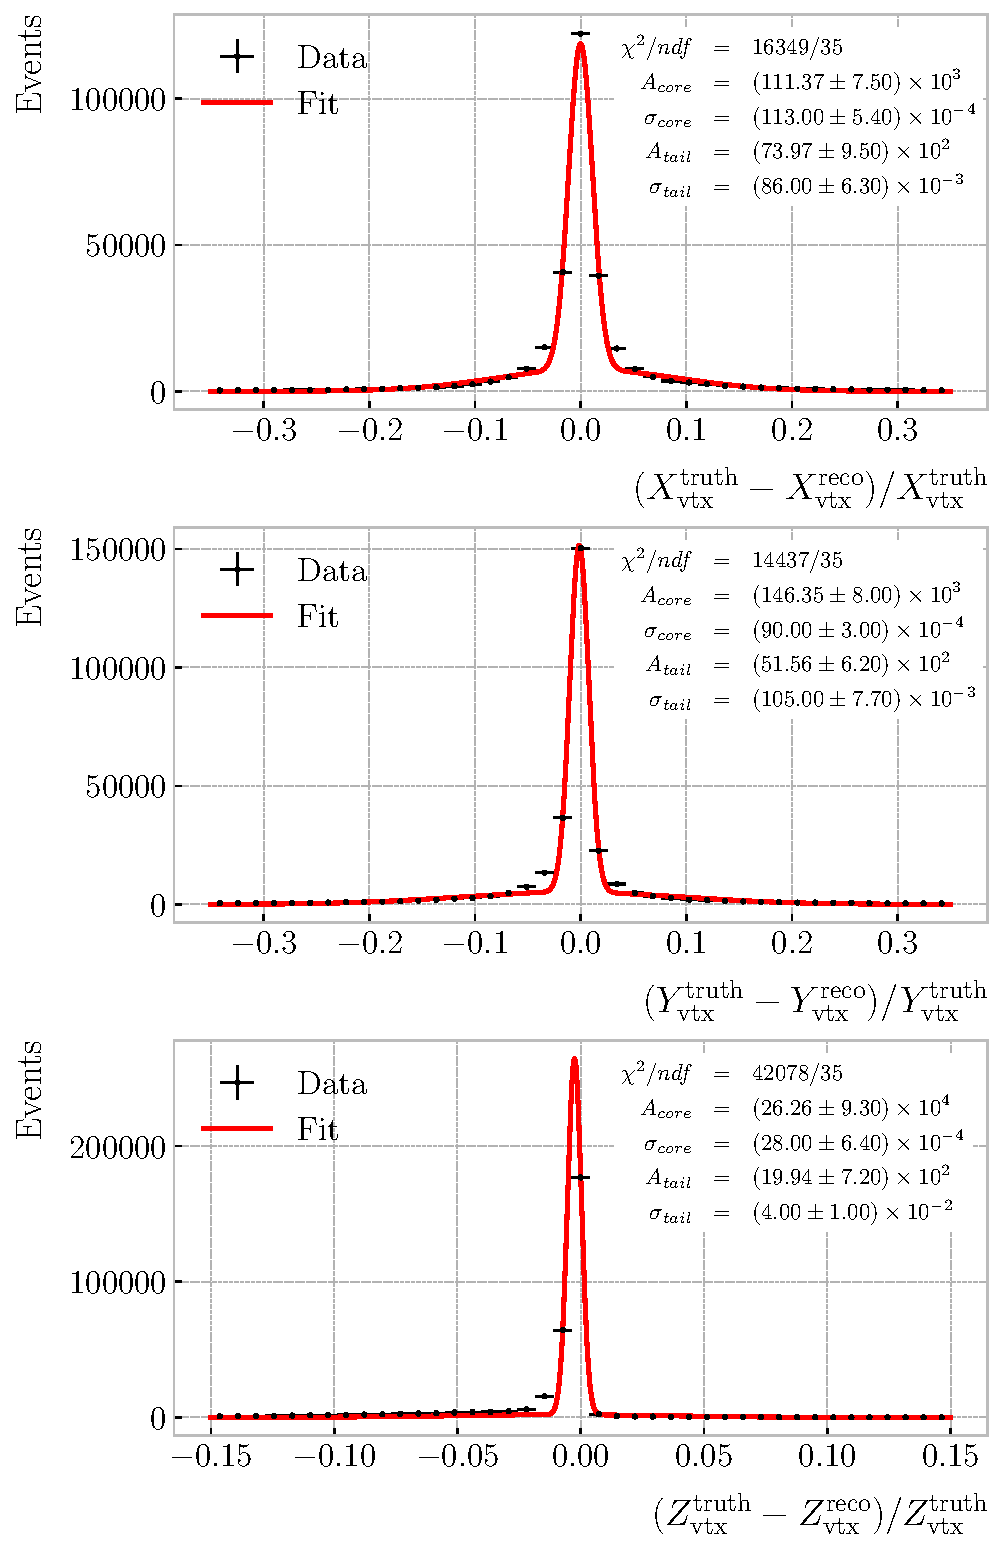
\includegraphics[width=.80\linewidth]{Images/GAr_selection/numuCC_muon_vtx_residuals.pdf}
    \caption[Fractional residual distributions for the position of the primary vertex in the $\nu_{\mu}$ CC selection.]{Fractional residual distributions for the position of the primary vertex in the $\nu_{\mu}$ CC selection. The best fits to a double Gaussian function are also shown (red lines).}
    \label{fig:numuCC_vertex_residuals}
\end{figure}

I also studied the performance of the $\nu_{\mu}$ CC selection as a function of the kinematic variables of the primary muon. As before, these metrics are only possible to compute for true $\nu_{\mu}$ CC events. The efficiency (top panels) and purity (bottom panels) as a function of the truth muon momentum (left) and beam angle (right) are shown in Fig. \ref{fig:numuCC_muon_kinematics}. One can see that there are some similarities in the behaviour of both metrics between the true neutrino energy and the muon momentum cases. This is to be expected, as these two variables are highly correlated. For the efficiency, there is a rapid increase at low momentum values until it peaks at around $1~\mathrm{GeV}/c$, after which it starts decreasing slowly. The purity remains relatively constant, with a slight drop towards high $p_{\mu}^{\mathrm{truth}}$ values. In the case of the muon angle, the decrease in efficiency at high $\theta_{\mu}^{\mathrm{truth}}$ is more noticeable. However, note that the number of events with backward-going muons is much smaller than those aimed towards the forward direction, as can be seen from the size of the vertical error bars. There is also a decline in the purity with the beam angle, but this effect is much smaller.

A byproduct of selecting the primary lepton in the interaction is the position of the reconstructed neutrino vertex candidate. Checking how the position of the selected reconstructed primary vertex and the true vertex position compare is needed to understand the validity of our method. Figure \ref{fig:numuCC_vertex_residuals} shows the distributions of fractional residuals between the truth and reconstructed vertex positions in the $X$ (top panel), $Y$ (middle panel), and $Z$ (bottom panel) directions. Performing a double Gaussian fit to the distributions (red lines), I estimate the reconstructed vertex resolution achieved with this method to be $1.62 \pm 0.08 \%$, $1.23 \pm 0.05 \%$, and $0.32 \pm 0.05 \%$ for the $X$, $Y$, and $Z$ directions, respectively. As expected, the resolution along the drift direction. However, the significant difference in resolution between the two transverse directions is worth noting. Not only the resolution is better for the $Z$ direction, but the layout of the residual distribution is highly asymmetrical. This may be related to the variability in the selection efficiency along that direction.

\begin{comment}
\begin{figure}[t]
    \centering
    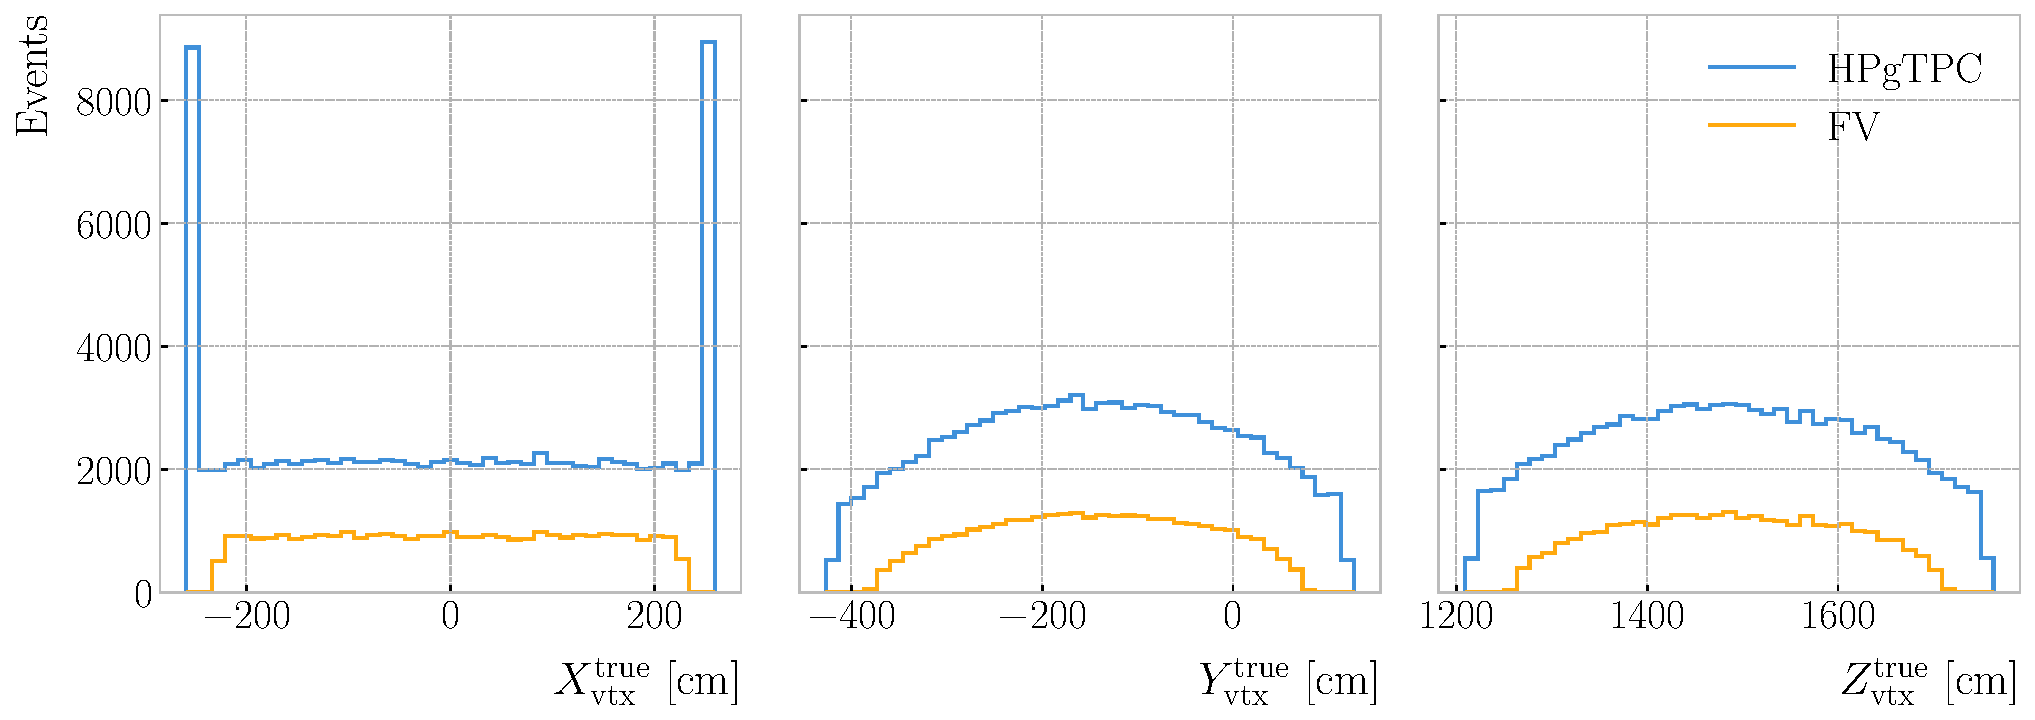
\includegraphics[width=.99\linewidth]{Images/GAr_selection/numuCC_true_vertex_position_fiducial.pdf}
    \caption[Distributions of the true $\nu_{\mu}$ CC vertex positions for the full HPgTPC and the FV.]{Distributions of the true $\nu_{\mu}$ CC vertex positions for the full HPgTPC volume (blue) and the optimised FV (yellow), given by $\Delta L_{\mathrm{FV}} = 30.0 ~ \mathrm{cm}$ and $\Delta R_{\mathrm{FV}} = 50.0 ~ \mathrm{cm}$.}
    \label{fig:numuCC_true_vertex}
\end{figure}
\end{comment}

\section{Charged pion identification}

Now that I have checked the robustness of the proposed $\nu_{\mu}$ CC selection, it can be used as a starting point for other, more convoluted, selections. One of the priorities of ND-GAr, as mentioned previously, is the identification of pions. With its lower tracking thresholds, ND-GAr is expected to do better regarding $\pi^{\pm}$ identification than the traditional LArTPCs, like ND-LAr. Moreover, it can make use of the different detector subcomponents to tag the charged pions.

\begin{figure}[t]
    \centering
    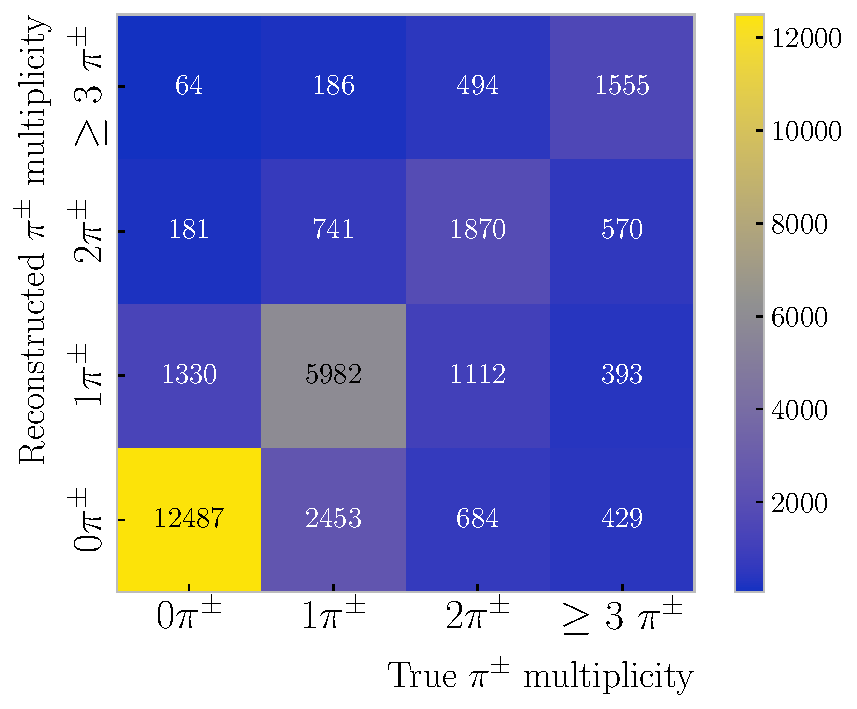
\includegraphics[width=.75\linewidth]{Images/GAr_selection/pion_selection_confusion_matrix.pdf}
    \caption[Distribution of events given their true and reconstructed $\pi^{\pm}$ multiplicity, for a given selection.]{Distribution of events given their true and reconstructed $\pi^{\pm}$ multiplicity, for the selection given by $p^{\mathrm{cut}}_{\mathrm{d}E/\mathrm{d}x} = p^{\mathrm{cut}}_{\mathrm{ToF}} = 0.50$, $\Delta^{\pi^{\pm}}_{\mathrm{d}E/\mathrm{d}x} = 0.20$, and $d^{\mathrm{cut}}_{\mu} = 50.0~\mathrm{cm}$.}
    \label{fig:pion_multiplicity_example}
\end{figure}

The $\nu_{\mu}$ CC selection provides a starting point for the pion identification. The first thing one can do is rule out the selected primary muon candidate. Then, by looking at the properties of the rest of the reconstructed particles, one can start the counting of the charged pions.

The two proton scores, the one based on the $\mathrm{d}E/\mathrm{d}x$ in the HPgTPC and the one obtained from the ToF measurement in the ECal, can be used to separate the protons from the sample of charged pions. By providing appropriate cuts for these, a good separation can be achieved.

Another source of information available is the $\mathrm{d}E/\mathrm{d}x$ of the track associated to the reconstructed particle. To select the charged pions, we can require that the measured mean $\mathrm{d}E/\mathrm{d}x$ is compatible with the expectation for a true $\pi^{\pm}$, in other words:
\begin{eqnarray}
    \left<\frac{\mathrm{d}E}{\mathrm{d}x}\right>_{\pi^{\pm}} \left(1 - \Delta_{\mathrm{d}E/\mathrm{d}x}^{\pi^{\pm}}\right) \leq \left<\frac{\mathrm{d}E}{\mathrm{d}x}\right>_{\mathrm{meas.}} < \left<\frac{\mathrm{d}E}{\mathrm{d}x}\right>_{\pi^{\pm}} \left(1 + \Delta_{\mathrm{d}E/\mathrm{d}x}^{\pi^{\pm}}\right),
\end{eqnarray}
where the parameter $\Delta_{\mathrm{d}E/\mathrm{d}x}^{\pi^{\pm}}$ measures the fractional variation one allows around the theoretical expectation. To obtain the expected mean $\mathrm{d}E/\mathrm{d}x$ of a charged pion with a given momentum, I use the ALEPH parametrisation with the parameter values obtained previously.

Also, as we are only interested in the primary pions, and because these are by definition close to the interaction vertex, one can apply an additional distance cut. Using the start position of the muon candidate, we can restrict the starting point of pions to a certain volume around the vertex.

Combining all these ideas, I propose the following procedure to identify the charged pions in an event:
\begin{enumerate}
    \item Apply $\nu_{\mu}$ CC selection.
    \item Disregard particle selected as primary muon.
    \item Remove particles with momentum below threshold.
    \item Select particles with proton $\mathrm{d}E/\mathrm{d}x$ score below threshold.
    \item Select particles with proton ToF score below threshold.
    \item Select particles with mean $\mathrm{d}E/\mathrm{d}x$ around the expected value for a pion.
    \item Remove particles with a distance between the start of the track and the primary vertex greater than the cut.
\end{enumerate}
The remaining particles after all these cuts are taken to be charged pion candidates.

\begin{figure}[t]
    \centering
    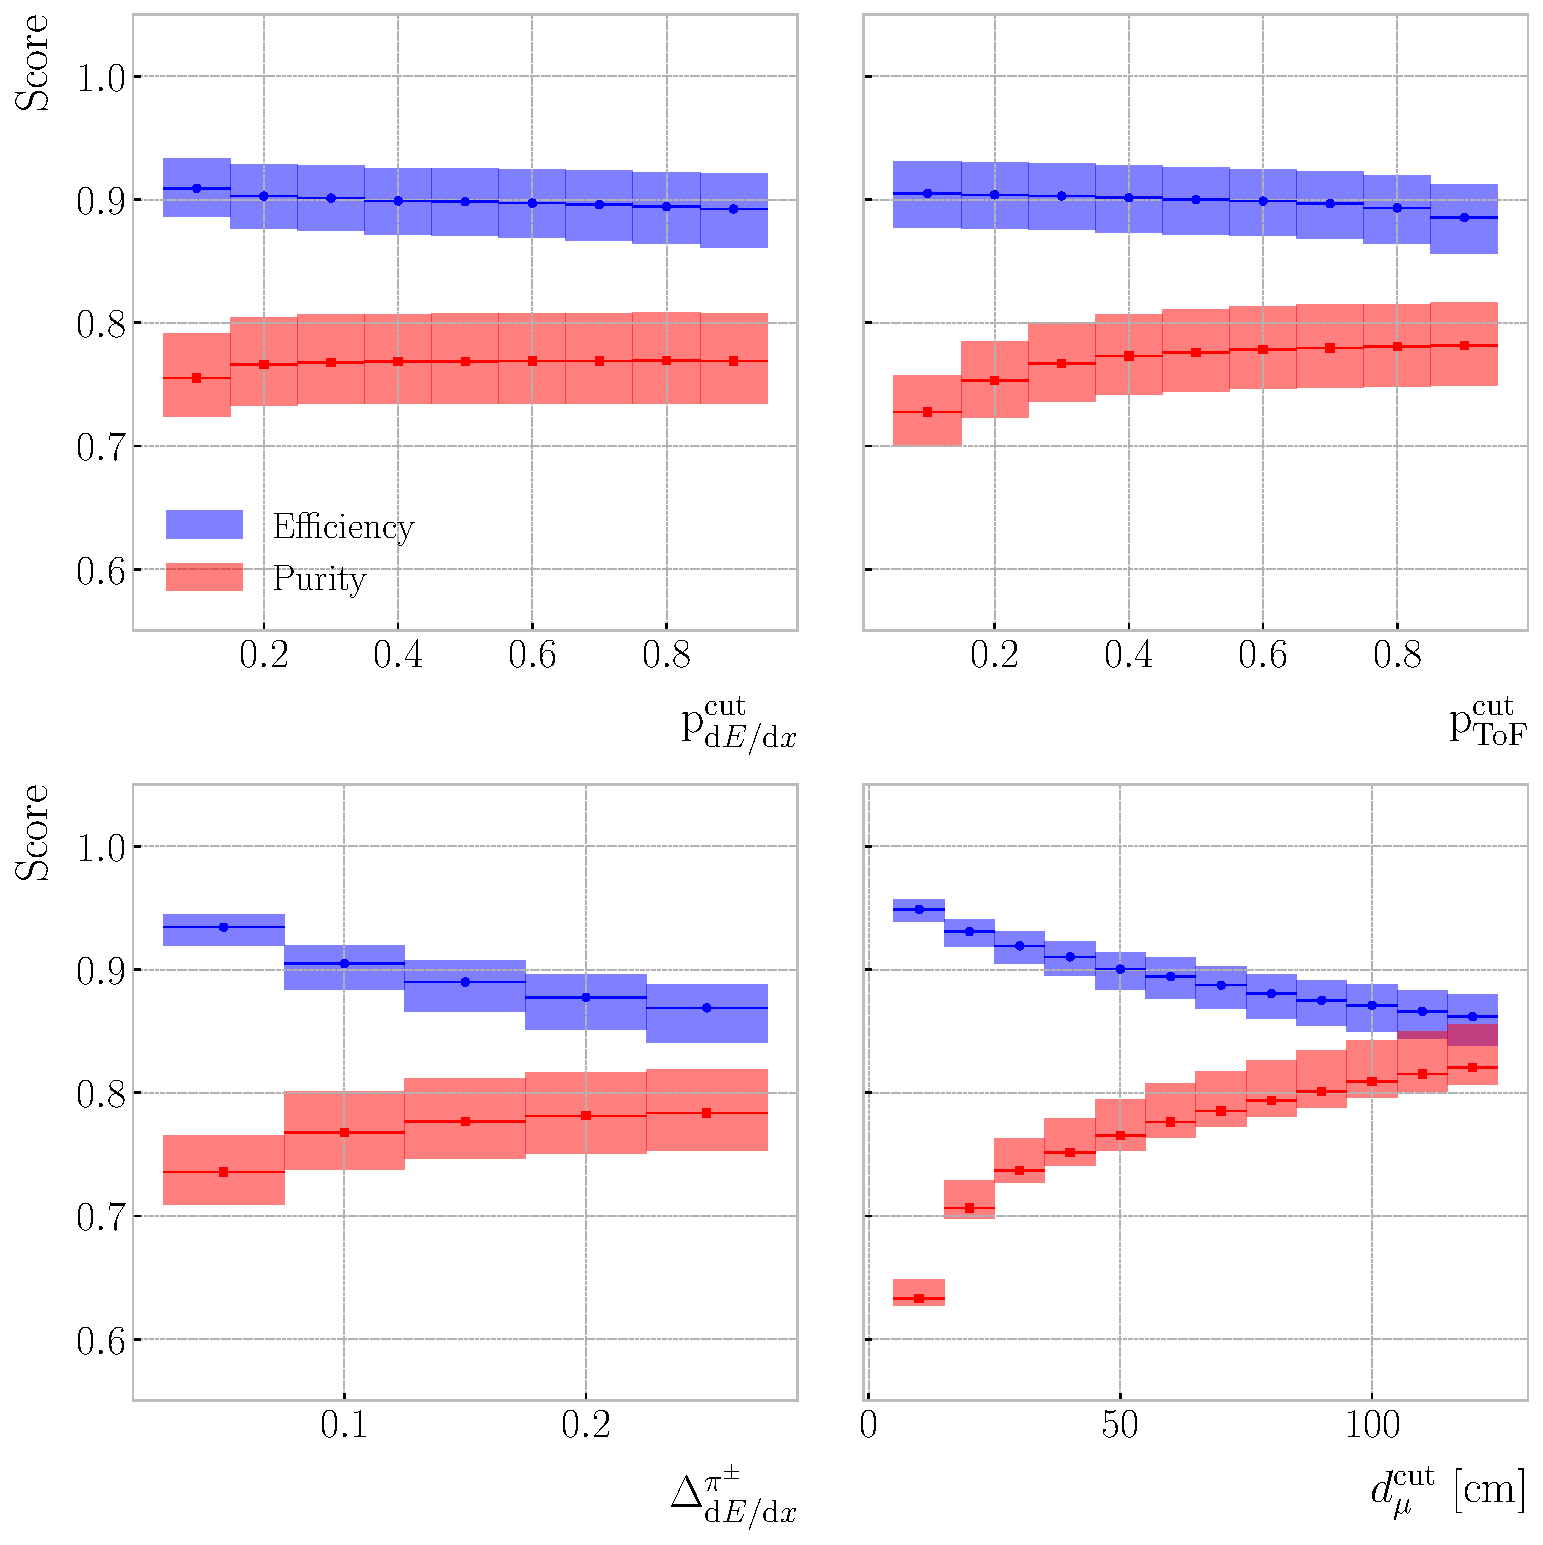
\includegraphics[width=.85\linewidth]{Images/GAr_selection/pion_selection_0_pions_metrics.pdf}
    \caption[Efficiency and purity for the $\nu_{\mu}$ CC $0\pi^{\pm}$ selection as a function of the different cuts.]{Efficiency (blue) and purity (red) for the $\nu_{\mu}$ CC $0\pi^{\pm}$ selection as a function of the proton $\mathrm{d}E/\mathrm{d}x$ score cut (top left panel), proton ToF score cut (top right panel), pion $\mathrm{d}E/\mathrm{d}x$ cut (bottom left panel), and distance to muon cut (bottom right panel). The height of the boxes represents the IQR of the conditional distributions, whereas the line corresponds to the median.}
    \label{fig:pion_selection_0_pions_metrics}
\end{figure}

This counting method depends on four cuts, denoted by $p^{\mathrm{cut}}_{\mathrm{d}E/\mathrm{d}x}$, $p^{\mathrm{cut}}_{\mathrm{ToF}}$, $\Delta^{\pi^{\pm}}_{\mathrm{d}E/\mathrm{d}x}$, and $d^{\mathrm{cut}}_{\mu}$ in order of appearance. The momentum threshold is necessary to compare with the true multiplicity. For values of the kinetic energy lower than $10-20~\mathrm{MeV}$, we do not expect to be able to tag individual pions. Such low energy particles just leave small traces in the TPC which, together with the busy environment of the neutrino interaction vertex, leaves one with no other option but to only account for their energy calorimetrically. As such, the true pion counting also features this momentum threshold.

I performed an optimisation of the charged pion counting by scanning the space of possible cut configurations. For the two proton scores, I let them vary between $0.10$ to $0.90$, in increments of $0.10$. Similarly, the parameter $\Delta^{\pi^{\pm}}_{\mathrm{d}E/\mathrm{d}x}$ takes values in the range $0.05-0.25$, with a step size of $0.05$. Finally, the distance cut changes in $10~\mathrm{cm}$ steps, from $10$ to $120~\mathrm{cm}$.

For each combination of selection cuts, I compare the true charged pion multiplicity given by GENIE with the number of charged pion candidates I count with this method, hereafter referred to as the reconstructed $\pi^{\pm}$ multiplicity. The result of this comparison is a matrix, with columns and rows indicating true and reconstructed charged pion multiplicity, respectively. An example of one of these matrices, obtained for a certain configuration of cuts, can be seen in Fig. \ref{fig:pion_multiplicity_example}. From these multiplicity matrices one can extract performance metrics, like efficiency, purity, and significance.

\begin{figure}[t]
    \centering
    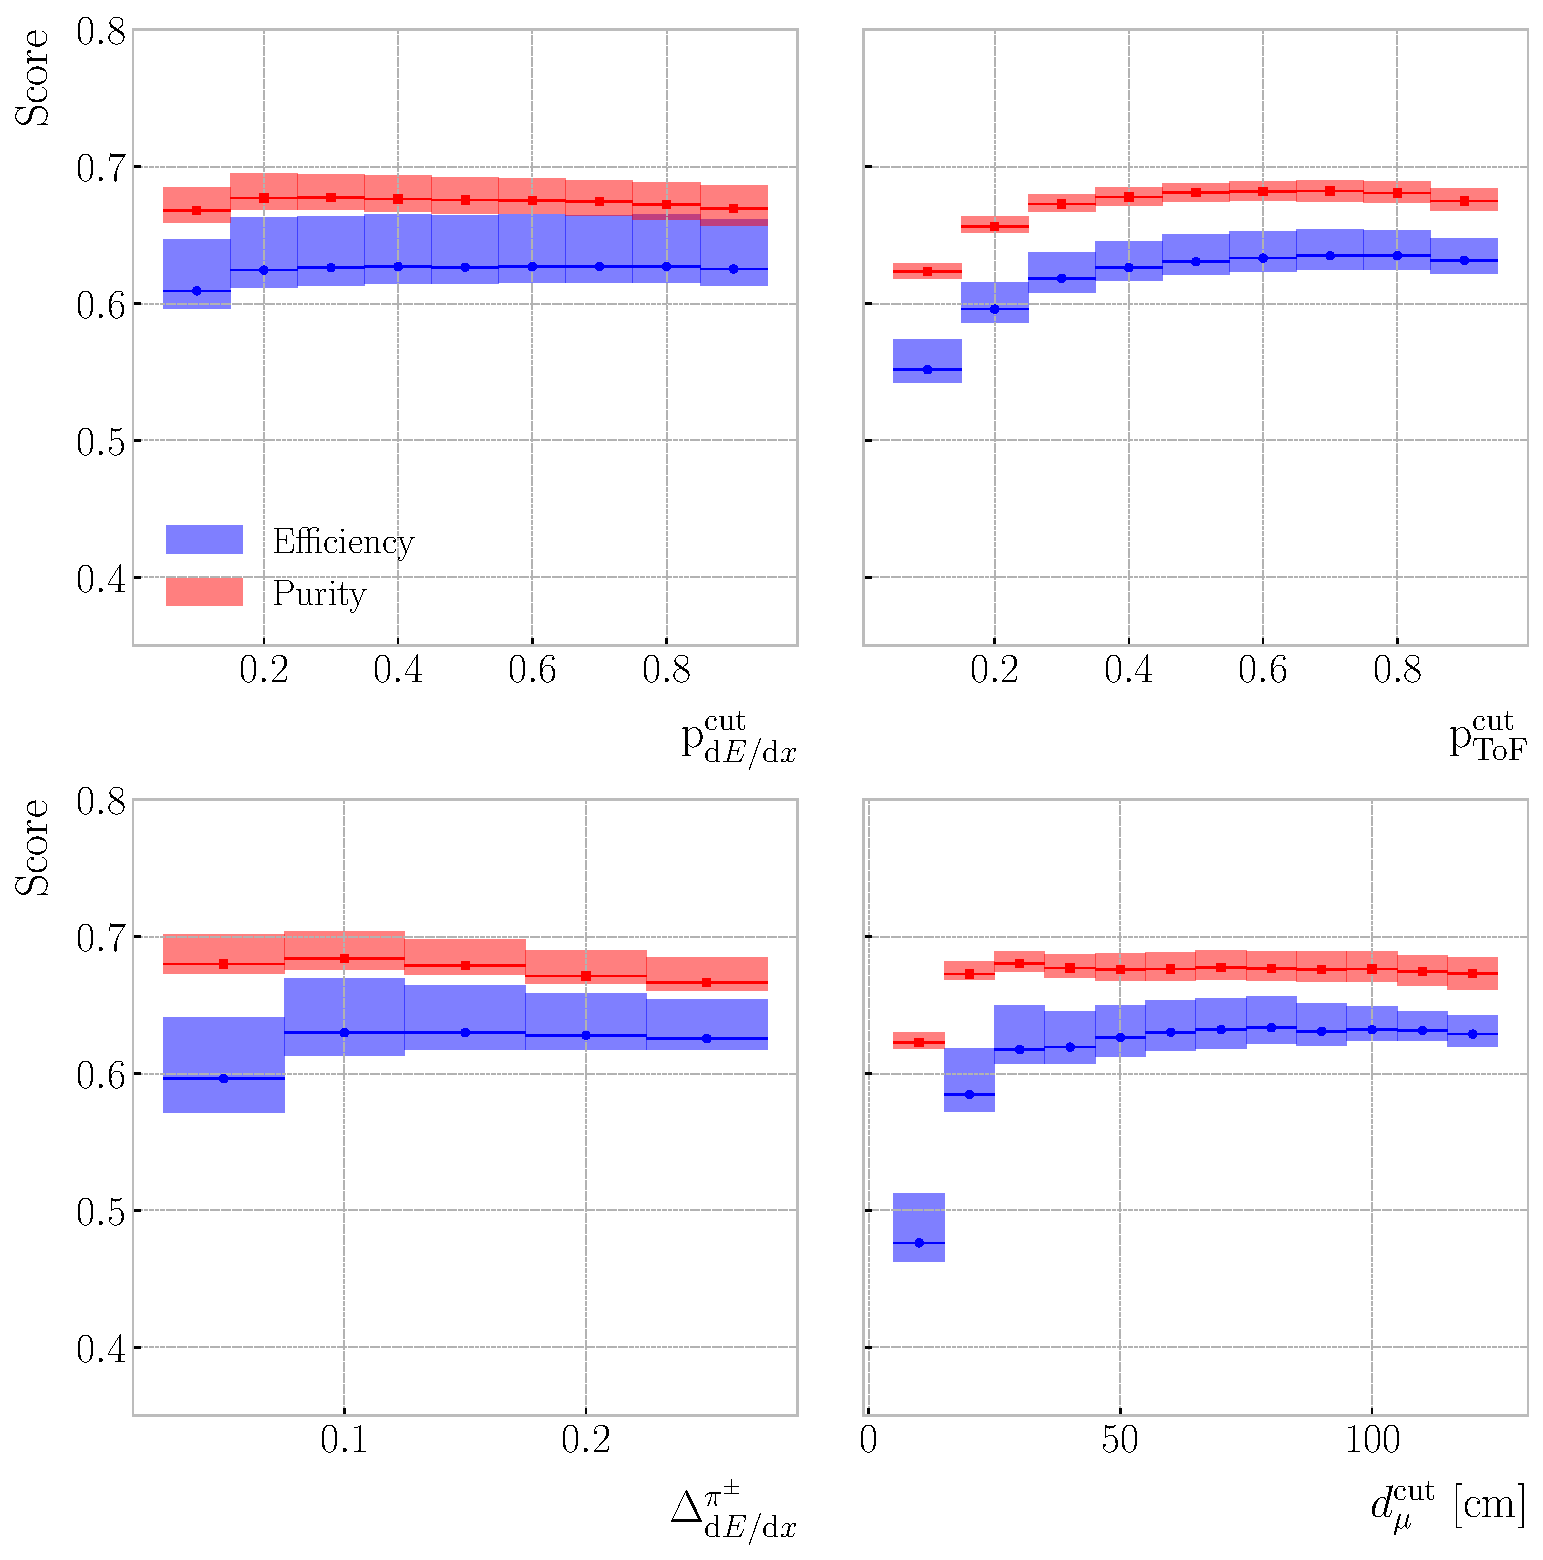
\includegraphics[width=.85\linewidth]{Images/GAr_selection/pion_selection_1_pions_metrics.pdf}
    \caption[Efficiency and purity for the $\nu_{\mu}$ CC $1\pi^{\pm}$ selection as a function of the different cuts.]{Efficiency (blue) and purity (red) for the $\nu_{\mu}$ CC $1\pi^{\pm}$ selection as a function of the proton $\mathrm{d}E/\mathrm{d}x$ score cut (top left panel), proton ToF score cut (top right panel), pion $\mathrm{d}E/\mathrm{d}x$ cut (bottom left panel), and distance to muon cut (bottom right panel). The height of the boxes represents the IQR of the conditional distributions, whereas the line corresponds to the median.}
    \label{fig:pion_selection_1_pions_metrics}
\end{figure}

Given a multiplicity matrix $\mathbf{M}$, the efficiency for the $i$-th multiplicity value can be computed as:
\begin{equation}\label{eq:efficiency_matrix}
    \left.\mathrm{Efficiency}\right|_{i} = \frac{M_{ii}}{\sum_{j} M_{ij}},
\end{equation}
or in other words, dividing the corresponding diagonal entry by the sum of all the entries in the same column. On the other hand, the purity is given by:
\begin{equation}\label{eq:purity_matrix}
    \left.\mathrm{Purity}\right|_{i} = \frac{M_{ii}}{\sum_{j} M_{ji}},
\end{equation}
which is just the ratio between the diagonal entry and the sum of the entries in the corresponding row. Similarly, the significance is obtained by taking the square root of the denominator in the previous expression:
\begin{equation}\label{eq:significance_matrix}
    \left.\mathrm{Significance}\right|_{i} = \left.\frac{S}{\sqrt{S+B}}\right|_{i} = \frac{M_{ii}}{\sqrt{\sum_{j} M_{ji}}}.
\end{equation}

Figures \ref{fig:pion_selection_0_pions_metrics} and \ref{fig:pion_selection_1_pions_metrics} show the efficiency (blue) and the purity (red) for the $\nu_{\mu}$ CC $0\pi^{\pm}$ and $1\pi^{\pm}$ selections, respectively, as a function of the different cut values. In the figures, each box represents the IQR of the conditional distribution for the fixed value of the corresponding cut, and the horizontal lines correspond to the medians. The first thing one notices is that the efficiency is always higher than the purity in the $0\pi^{\pm}$ selection, while the opposite is true for the $1\pi^{\pm}$ selection. Also, it is clear that the range within these metrics fluctuate in the $0\pi^{\pm}$ selection is significantly higher than it is for the $1\pi^{\pm}$ case. This shows that it is easier to assess that no charged pions are present in the event than actually tagging them.

For the $\nu_{\mu}$ CC $0\pi^{\pm}$ selection, the performance metrics follow the expected tendency. As the purity grows with a cut value, the efficiency decreases. Interestingly, this is not the case fot the $1\pi^{\pm}$ selection, where both efficiency and purity follow roughly the same trends along the different cuts. This makes sense when one comprehends that this is not a traditional cut-based selection, but more of a counting exercise. Some restrictive cut configurations will not tag any particles as pions. On the contrary, loose cuts will render every particle as a $\pi^{\pm}$. Therefore, when looking at a specific multiplicity, the relation between the cut value and the performance metrics is not obvious. Thus, sometimes efficiency and purity can both increase, as the cuts refine the definition of a reconstructed pion.

\begin{figure}[t]
    \centering
    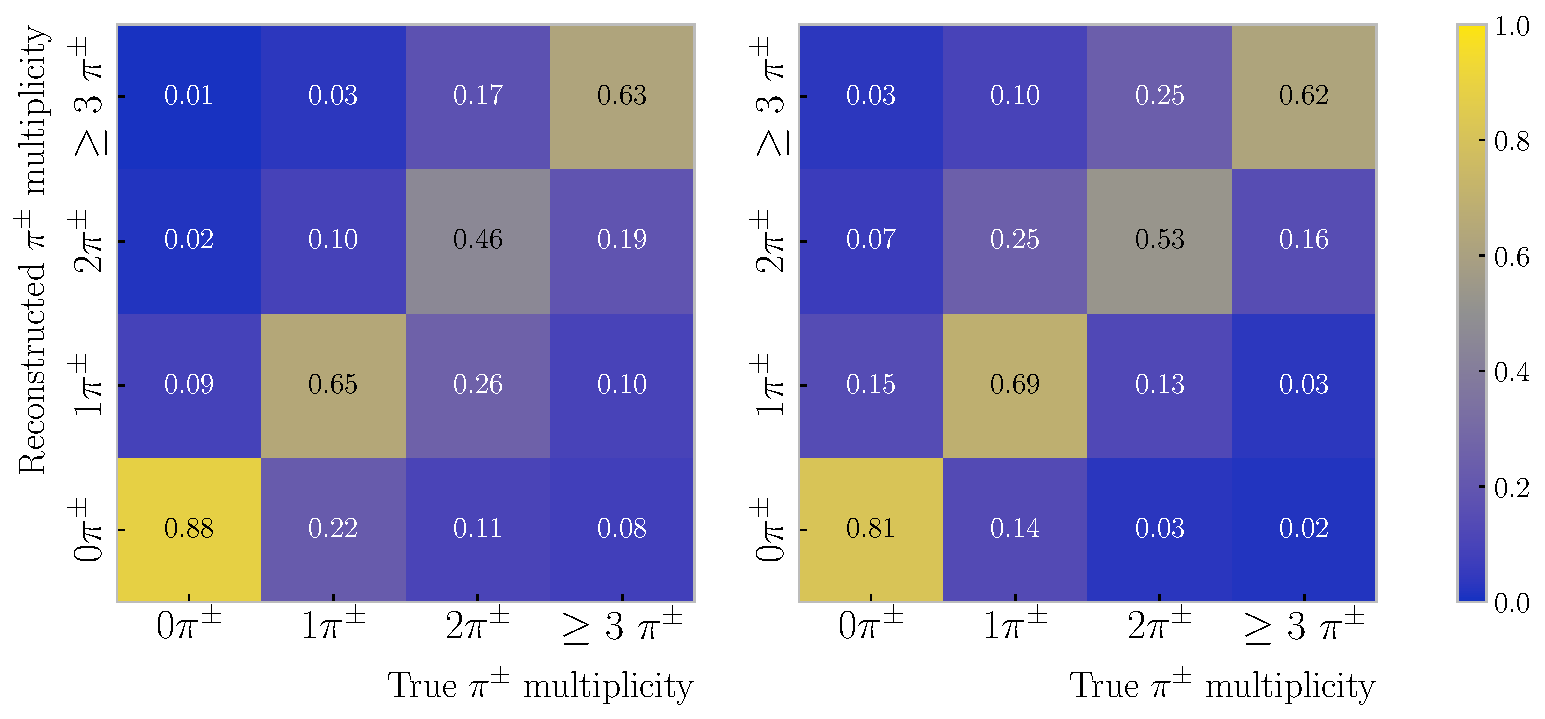
\includegraphics[width=.99\linewidth]{Images/GAr_selection/pion_selection_metrics_matrix_max_significance.pdf}
    \caption[Row and column normalised distributions of events given their true and reconstructed $\pi^{\pm}$ multiplicity, for the selection that maximises the significance of the $\nu_{\mu}$ CC $1\pi^{\pm}$ selection.]{Distribution of events given their true and reconstructed $\pi^{\pm}$ multiplicity, both column-wise (left panel) and row-wise (right panel) normalised, for the selection that maximises the significance of the $\nu_{\mu}$ CC $1\pi^{\pm}$ selection. The column normalisation yields the efficiency in the diagonal entries, whereas the row normalisation reveals the purity.}
    \label{fig:pion_selection_metrics}
\end{figure}

To have a working point for our studies, I chose the cut configuration that yields the maximum significance for the $\nu_{\mu}$ CC $1\pi^{\pm}$ selection. Of course, other cuts would be more appropriate in certain scenarios. However, this provides us with a starting point to understand the performance of the selection. A significance of $66\pm7$ for the $1\pi^{\pm}$ selection is achieved for the cut values $p^{\mathrm{cut}}_{\mathrm{d}E/\mathrm{d}x} = 0.30$, $p^{\mathrm{cut}}_{\mathrm{ToF}} = 0.70$, $\Delta^{\pi^{\pm}}_{\mathrm{d}E/\mathrm{d}x} = 0.10$, and $d^{\mathrm{cut}}_{\mu} = 110.0~\mathrm{cm}$.

Figure \ref{fig:pion_selection_metrics} shows the multiplicity matrices resulting from this optimised $\nu_{\mu}$ CC $1\pi^{\pm}$ selection. Although both matrices are produced with the same selection cuts, one is column normalised (left panel), whereas the other is row normalised (right panel). It follows from the definitions in Eqs. (\ref{eq:efficiency_matrix}) and ((\ref{eq:purity_matrix})) that the diagonal entries of these matrices correspond to the efficiencies and the purities, respectively, for each of the possible charged pion multiplicity selections.

\begin{figure}[t]
    \centering
    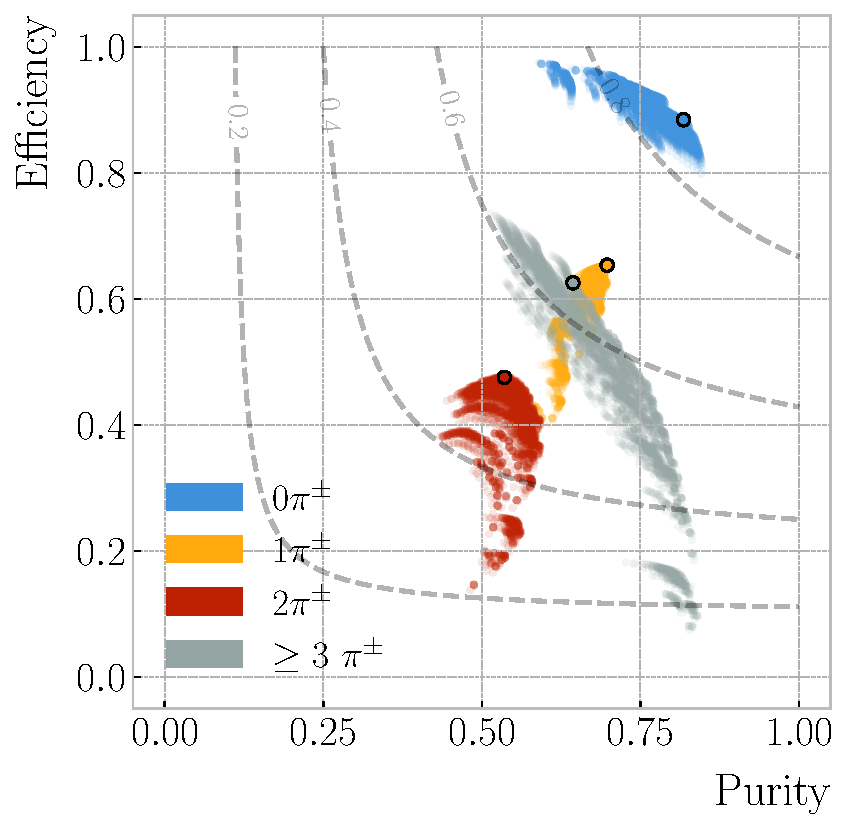
\includegraphics[width=.70\linewidth]{Images/GAr_selection/pion_selection_all_in_one_purity_vs_efficiency.pdf}
    \caption[Purity versus efficiency achieved for the different cut configurations explored separated by the various $\nu_{\mu}$ CC $N\pi^{\pm}$ selections.]{Purity versus efficiency achieved for the different cut configurations explored separated by the various $\nu_{\mu}$ CC $N\pi^{\pm}$ selections. The outlined points indicate the state for each possible multiplicity when using the configuration that maximises the significance of the $\nu_{\mu}$ CC $1\pi^{\pm}$ selection. The contours indicate the surfaces of equal $F_{1}$-score.}
    \label{fig:pion_purity_vs_efficiency}
\end{figure}

An additional check to make is understand how this configuration performs when applied to the other selections, like $\nu_{\mu}$ CC $0\pi^{\pm}$, and how it compares to the other possible configurations. A comparison between the different pion multiplicity selections, indicated with colours, in the purity versus efficiency space is shown in Fig. \ref{fig:pion_purity_vs_efficiency}. For each of the possible multiplicity choices, the performance obtained for the $1\pi^{\pm}$ optimised selection is indicated by an outlined point. From this, one can see that the selected configuration performs reasonably well, within the limits of what can be achieved in each case, across the different multiplicities.

\subsection[\texorpdfstring{$\nu_{\mu}$}{numu} CC \texorpdfstring{$1\pi^{\pm}$}{1pi} selection]{\boldmath\texorpdfstring{$\nu_{\mu}$}{numu} CC \boldmath\texorpdfstring{$1\pi^{\pm}$}{1pi} selection}

\section{Neutral pion identification}

\begin{figure}[t]
    \centering
    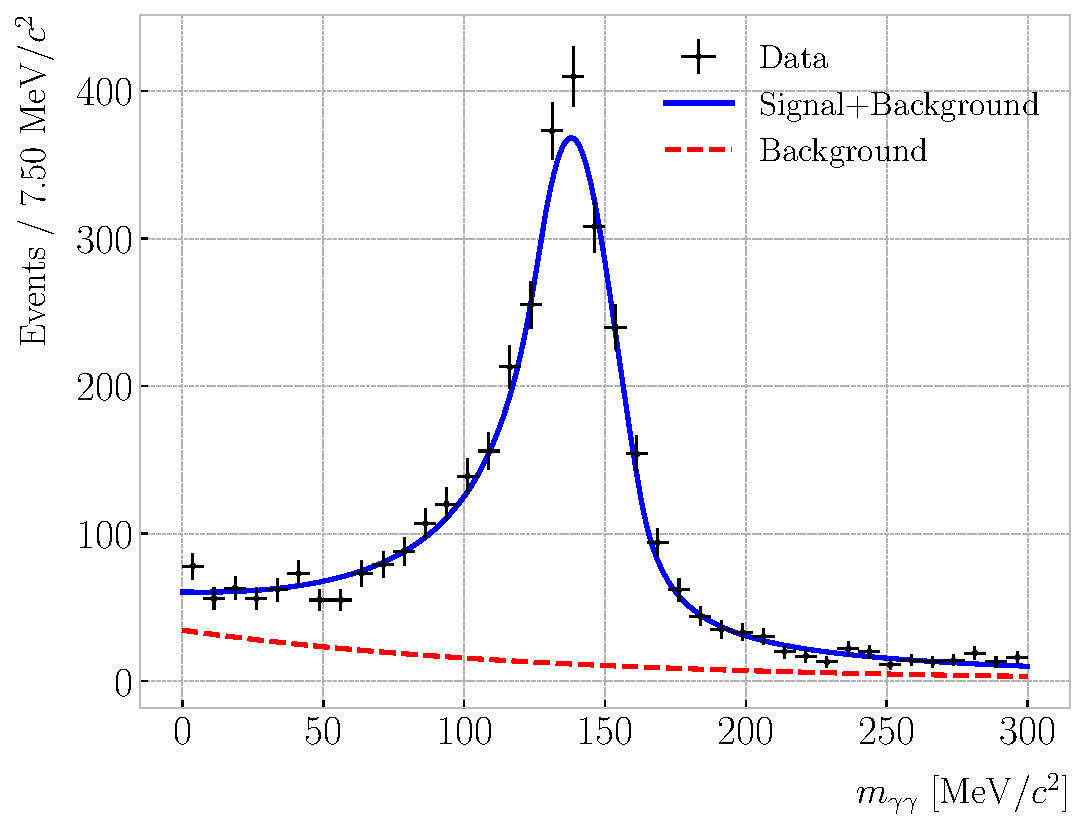
\includegraphics[width=.80\linewidth]{Images/GAr_selection/numuCC_1pizero_selection_biased.pdf}
    \caption[Invariant mass distribution obtained for the unassociated ECal cluster pair in the event with the value closest to the true $\pi^{0}$ mass.]{Invariant mass distribution obtained for the unassociated ECal cluster pair in the event with the value closest to the true $\pi^{0}$ mass. The best fits for signal plus background (solid blue line) and background only (dashed red line) are also shown.}
    \label{fig:pion_selection_metrics}
\end{figure}

\section{Systematic uncertainties}

\subsection{Flux uncertainties}

% Introduction
The neutrino flux prediction is affected by systematic uncertainties arising from two sources: the uncertainties in the production of hadrons in the target and the uncertainties in the design parameters of the beamline itself. These fluxes and their uncertainties are generated with the G4LBNF simulation \cite{DUNE2020TDR2}, a Geant4 implementation of the LBNF beamline, and the Package to Predict the FluX (PPFX) framework, originally developed for MINERvA \cite{Golan2016}.

% Hadron-production uncertainties
The hadron production uncertainties are associated to the kinematic distributions of the hadrons produced when the protons interact with the carbon target, as well as the possible interactions of the hadrons with the beamline materials. The PPFX package estimates these uncertainties by performing a number of random throws of the production model parameters \cite{Bashyal2017}. This way, different predictions of the LBNF flux are generated, which can be compared to the nominal prediction to build a matrix of the covariances between neutrino energies, flavours and running modes (either FHC or RHC). The resulting hadron production uncertainties are described by the eigenvectors associated to the largest eigenvalues in this matrix, obtained performing a PCA analysis.

% Beamline instrumentation uncertainties
The other set of uncertainties affecting the neutrino flux prediction come from the limited precision with which we know the parameters of the different components in the beamline. These include the specifications of the target, the dimensions of the decay pipe, and the current and alignment of the magnetic horns. The effects on the flux predictions of these uncertainties are estimated using the G4LBNF simulation. For each of the parameters, the simulation runs with said parameter shifted by $\pm 1\sigma$ from the nominal value, and the resulting flux prediction is compared to the nominal one.

\subsection{Cross section uncertainties}

\subsection{Detector uncertainties}